%% 
%% This is file `squelette-rr.tex',
%% generated with the docstrip utility.
%% 
%% The original source files were:
%% 
%% RR.dtx  (with options: `sample')
%% ********************************************************************
%% Copyright (C) 1997-1999 2004 2006-2011 INRIA/APICS/MARELLE by Jose' Grimm
%% This file may be distributed and/or modified under the
%% conditions of the LaTeX Project Public License, either version 1.3
%% of this license or (at your option) any later version.
%% The latest version of this license is in
%% http://www.latex-project.org/lppl.txt
%% and version 1.3 or later is part of all distributions of LaTeX
%% version 2003/12/01 or later.
%% An archive of the software can be found at
%% ftp://ftp-sop.inria.fr/marelle/RR-INRIA

\documentclass[twoside]{article}
\usepackage[a4paper]{geometry}
\usepackage{amsmath,amsfonts,amssymb}
\usepackage[latin1]{inputenc} % ou \usepackage[utf8]{inputenc}
\usepackage[T1]{fontenc} % ou \usepackage[OT1]{fontenc}
\usepackage{pgf}
\usepackage{tikz}
\usetikzlibrary{arrows,automata}


\usepackage{RR}
% \usepackage{hyperref}
\usepackage{flexisym}
\usepackage[linesnumbered,ruled]{algorithm2e}
% \usepackage{caption}
\usepackage{subcaption}
\usepackage[biblabel,nomove]{cite}
\bibliographystyle{naturemag}
%% \usepackage[frenchb]{babel} % optionnel
\usepackage[labelfont={bf,sf},%
labelsep=period,%
justification=raggedright]{caption}
\usepackage[colorlinks=true, allcolors=blue]{hyperref}
\usepackage{xcolor}
\usepackage{float}
\usepackage[titletoc,toc,title]{appendix}
\usepackage{amsthm}
\newtheorem{theorem}{Theorem}
\newcounter{fig}\setcounter{fig}{0}
\RRNo{1}
%% \RTNo{0703}
%% 
%% date de publication du rapport
\RRdate{July 2016}
%% 
%% Cas d'une version deux
%% \RRversion{2}
%% date de publication de la version 2
%% \RRdater{November 2008}
%% 
\RRauthor{% les auteurs
  % Premier auteur, avec une note
  Alexandre Moreau%\thanks{Footnote for first author}%
  % note partag\'ee (optionnelle)
  \thanks[sfn]{Shared foot note}%
  % \and entre chaque auteur s'il y en a plusieurs
  \and
  Luc Giraud%\thanks{Footnote for second author}%
  % r\'ef\'erence \`a la note partag\'ee
  \thanksref{sfn}
  % liste longue pour tests de mise en page
  \and Emmanuel Agullo%\thanks{etc} \and Andr\'e Lichnerowicz
  % \and Marcel-Paul Sch\"utzenberger \and Jacques-Louis Lions
}
%% Ceci apparait sur chaque page paire.
\authorhead{Alexandre Moreau}% \& Louarn \& others}
%% titre francais long
\RRtitle{Rapport de 3 mois}
%% English title
\RRetitle{Adaptive fault detection criterion for the generalized
  minimal residual method}
%% 
\titlehead{Rapport}
%% 
% \RRnote{This is a note}
% \RRnote{This is a second note}
%% 
%% \RRresume{Ce document montre comment utiliser le style RR.sty.
%% Pour en savoir plus, consulter le fichier RR.dvi ou RR.pdf.
%% D\'efinissez toujours les commandes avant utilisation.
%% }
\RRabstract{
  We have studied the impact of transient soft errors in the application of the matrix
vector product or in the preconditioner of preconditioned GMRES. We have analyzed 
those faults and we are able to successfully correlate those faults to the framework
of inexact GMRES theory. We have derived a heuristic to detect faults. This
heursitic is extremely robust to detect faults for GMRES and left-preconditioned
GMRES and pretty robust in the case of right-preconitioned GMRES. An analysis
on the set up of the heurisitcs furthermore identified the critical parameter ($y_{l,k}$)
that we had to approximate in our heuristic and that may lead to miss a few faults.
  % As the computational performance of current HPC systems increases, the
  % mean time between failures (MTBF) decreases, down to a time comparable to or lower than the application execution time. Methods aiming at improving resiliency of
  % such systems and ensuring correct executions include algorithm-based
  % fault tolerance (ABFT). This paper focuses on the effects of transient
  % faults (bit-flips on temporary registers) occurring in GMRES executions,
  % and proposes a cheap numerical test to be added to the GMRES algorithm in
  % order to detect whether or not the convergence to the target accuracy has
  % been altered by a fault.
}

%% 
%% \RRmotcle{calcul formel, base de formules,  %mots-cl\'es sans rapport
%% protocole, diff\'erentiation automatique, % les uns avec les autres
%% g\'en\'eration de code,  mod\'elisation, lien symbolique/num\'erique,
%% matrice structur\'ee, r\'esolution de syst\`emes polynomiaux}
%% \RRkeyword{}
%% 
%% \RRprojet{Apics}  % cas d'un seul projet
\RRprojets{HiePACS}
%% 
%% \URLorraine % pour ceux qui sont \`a l'est
%% \URRennes  % pour ceux qui sont \`a l'ouest
%% \URRhoneAlpes % pour ceux qui sont dans les montagnes
%% \URRocq % pour ceux qui sont au centre de la France
%% \URFuturs % pour ceux qui sont dans le virtuel
%% \URSophia % pour ceux qui sont au Sud.
%% 
\RCBordeaux % centre de recherche Bordeaux - Sud Ouest
%% \RCLille % centre de recherche Lille Nord Europe
%% \RCParis % Paris Rocquencourt
%% \RCSaclay % Saclay \^Ile de France
%% \RCGrenoble % Grenoble - Rh\^one-Alpes
%% \RCNancy % Nancy - Grand Est
%% \RCRennes % Rennes - Bretagne Atlantique
%% \RCSophia % Sophia Antipolis M\'editerran\'ee

\DeclareMathOperator*{\argmin}{arg\,min}


%% 
\begin{document}
%% 
\makeRR   % cas d'un rapport de recherche
%% \makeRT % cas d'un rapport technique.
%% a partir d'ici, chacun fait comme il le souhaite

\tableofcontents

\newcommand{\allOne}{\bf{1}}
\newcounter{grecounter}
\newcounter{porescounter}

\section{Introduction}
The current trend to improve supercomputers' performance is to increase the component count while reducing their size. Future exascale systems will gather several millions of tiny CPU cores, which will drive the error rate up to many times per day. This issue is already taking place in some present petascale systems, that experience up to 3 failures per day (according to The Computer Failure Data Repository\cite{CFDR}, LANL). In case of a failure, an application without any fault tolerance mechanism may either stop or silently terminate with an incorrect output, which can have serious consequences in some applications. For this reason, we study the impact of faults and explore strategies to enhance the fault tolerance of particular applications in a specific context described below. 

Errors can be classified into two types, hard errors and soft errors. Hard errors are permanent and unrecoverable errors, for instance a system crash or a broken component, whereas soft errors are silent data corruptions that usually do not affect the system reliability, but may lead to incorrect results. In the following, we focus on the study of soft error tolerance.

Several schemes have been designed to enhance HPC system resiliency to soft errors. On one hand, hardware mechanisms usually relying on the addition of redundancy in the circuits are being used, but may be too costly in terms of hardware and energy to be systematically applicable in the future. On the other hand, software schemes are often more flexible and provide fault tolerance at lower cost.

Software schemes may be system-wide or at the application level. The standard system-wide method is Checkpoint/Restart: the system state is periodically saved into a safe memory storage, and a rollback is performed from a previous correct state whenever an incorrect state is detected. However this approach becomes expensive as the system size increases,  and may not be applicable in the long term as the mean time between failures (MTBF) gets closer and closer to the mean time to repair (MTTR). Moreover, it still requires a reliable fault detection mechanism. At the application level, this method is also being used and usually benefits from much smaller sized states, enabling more frequent checkpoints and shorter recovery times.

Other approaches at the application level include Algorithm Base Fault Tolerance (ABFT) such as check-sum based techniques, introduced by Kuang-Hua Huang and J. A. Abraham in \cite{checksum} and usually provide fault tolerance at lower cost and hardware overhead than standard application level schemes. More recently, studies on the algorithms numerical properties as well as floating point analysis have been used to provide evidences and quantify the impact of any potential perturbation occurring during the algorithm execution. More information about the current state of the art of the resilience in HPC can be found in \cite{Cappello:2014:TER:2983586.2983587}.

One of the most important and time-consuming kernel in numerical schemes is the solution of large sparse linear systems. One popular algorithm for solving such systems it the generalized minimum residual (GMRES) algorithm \cite{gmres}. 
In this report, we analyze the impact of soft-errors on the convergence of GMRES and deduce a new, robust fault-detection mechanism.

The rest of the report is organized as follows. In Section 2, the GMRES algorithm is described, in particular the variants we are interested in (full-GMRES, with and without preconditioner). In Section 3, the method, definitions and assumptions used throughout the numerical experiments are detailed. In Section 4, the impact of faults in GMRES is empirically studied. In Section 5, an analysis of the error introduced by faults is proposed, to quantify their impact and predict their influence on the convergence. In Section 6, an oracle-based detection scheme is described and evaluate. In Section 7, a more practical implementation of the detection scheme, based on some approximations, is proposed and evaluated. Finally a discussion on the results and concluding remarks are given.


\section{Solving linear systems of equations in HPC}
Large computational problems tackled by HPC systems often arise out of complex phenomenon models. To dispose of powerful mathematical tools, most of those models are linear or are linearized so that the innermost calculation reduces to the solution of the linear system of equations of the form
$$
A x = b \text{.}.
$$
where $A \in \Bbb{R}^{n\times n}$ and $b\in \Bbb{R}^n$ are known and $x \in \Bbb{R}^n$  is to be found with $n \gg 1$ up to a few tens of millions.

% as they rely on linear operators only, such as matrix-vector product, and can be reduced to the equation $A x = b$, where the matrix A and vector b are known, and the vector solution $x$ is to be found.
Several methods for computing a good solution to this equation are available, separated in two classes of algorithms. On one hand, direct solvers based on Gaussian elimination \cite{direct_solver} are very robust and provide an accurate solution in term of backward error~\cite{hig:02} 
% provide the exact (modulo rounding errors) solution $x$ 
at the end of the computation. On the other hand iterative solvers are given a first approximation $x_0$ of the solution $x$ as an additional parameter, and compute a sequence $(x_i)$ of improving approximations until the target accuracy is reached. In certain situations, the iterative methods have proved to be more practical than the direct ones, especially when the problem size is large, in which case direct methods can be prohibitively expensive. Depending on the structure and numerical properties of matrix A, some iterative methods will perform better than others. In particular, when A is a large, sparse and non-singular matrix, Krylov methods are particularly adapted. When the matrix A is non-symmetric, GMRES~\cite{gmres} is among the best known Krylov method to use~\cite{Saad:2003}.

\subsection{Krylov methods}
All Krylov methods designed to solve a linear system $Ax = b$ have in common the construction of the Krylov space of order i associated to A and b: $$\mathcal{K}_i(A, b) \equiv \text{span(}b, Ab, ..., A^{i-1}b\text{)} \text{.}$$ The reason behind the use of such a space is derived from the Cayley-Hamilton theorem, which implies that $A^{-1}$ can be expressed as a linear combination of powers of $A$. Consequently the solution $x = A^{-1}b$ belongs to $\mathcal{K}_i(A, b)$ for r large enough. The basis $\{b, Ab, A^2b...\}$ is iteratively computed using repeated matrix-vector product, until the distance between the spanned Krylov space and the solution is small enough. The solution $x$ can then be efficiently approximated inside this small-sized space. However, the basis vectors quickly become linearly dependent, which usually requires the use of some orthogonalization scheme to enhance the numerical stability.

\subsection{The GMRES algorithm}

The GMRES method (Algorithm \ref{alg:gmres}) was first described in 1986 by Saad and Schultz \cite{gmres} and is one of the most popular Krylov method for solving non-symmetric linear systems. It relies on the repetition of the Arnoldi iteration, which recursively generates an orthonormal basis $V_i = \{v_0, v_1, ... v_{i}\}$ for $\mathcal{K}_i(A, b)$ to project the initial problem $A x = b$ onto. The first Arnoldi vector $v_0$ is initialized to the first residual normalized $v_0 = r_0/\|r_0\| = (A x_0 - b) / \|A x_0 - b\|$ (line 2-4) and the recursive relation maintained throughout the algorithm is $$AV_i = V_{i+1}H_i \text{.}$$ where $H_i$ is an upper Hessenberg rectangular matrix of size $i+1 \times i$ produced by the orthonormalization scheme. The most widely used scheme is the modified Gram-Schmidt process (line 8-13), although variants using the classical Gram-Schmidt or the Householder process also exist but are numerically less stable or more expensive. The initial least-square problem of minimizing the residual norm $\|r\| = \|A x  - b\|$ becomes equivalent to a new least-square problem, easier to solve thanks to the structure and size of matrix $H_i$:
\begin{equation}\label{eq:minNomr}
  \argmin_{\mathbf{x} \in \mathcal{K}_i(A, b)} \|A \mathbf{x} - b\| = \argmin_{\mathbf{y}\in \Bbb{R}^i}\|\beta e_1 - H_{i} \mathbf{y}\| \text{ with } e_1 = [1, 0,...0]^T \text{ and } \beta = \|r_0\| \text{.}
\end{equation}
The upper-Hessenberg matrix $H$ can be efficiently transformed into an upper-triangular matrix, using QR factorization (for instance Givens rotations or Householder), to solve the new least-square problem using back substitution \cite{govl:96} (line 14). The Arnoldi process is repeated until the computed residual reaches the target accuracy, which requires at most n iterations in exact arithmetic, and the initial problem solution is expressed back into the initial basis using $x = x_0 + V_i y_i$ (line 17) where $y_i$ is the solution of Equation~\eqref{eq:minNomr}.

\begin{algorithm}
  \SetKwInOut{Input}{Input}
  \SetKwInOut{Output}{Output}
  \SetKwInOut{Parameter}{Parameter}
  \SetKwInOut{Break}{Break}
  
  \underline{GMRES} $(A, b, x_0, \varepsilon)$\;
  \Input{$A$ ($n \times n$ matrix), $b$ (size n vector), $x_0$ (size n vector)}
  \Parameter{$\varepsilon$ (target accuracy) }
  \Output{$x$ so that $\frac{\|A x - b\|}{\|b\|} < \varepsilon$}
  $r_0 \leftarrow Ax_0 - b$\;
  $ \beta \leftarrow \|  Ax_0 - b \|$\;
  $v_0 \leftarrow \frac{r_0}{\beta}$\;
  $e_1 \leftarrow [1, 0,..., 0]$\;
  \For{$i\leftarrow 0$ \KwTo $n-1$}
  {
    \tcp{Arnoldi iteration}
    $w \leftarrow A \cdot v_i$ \tcp*[f]{Compute the next Arnoldi vector}
    
    \For(\tcp*[f]{Orthonormalize w against}){$k\leftarrow 0$ \KwTo $i$} 
    {
      $h_{k,i} \leftarrow w^H v_k $ \tcp*[f]{all previous Arnoldi vectors}
      
      $w \leftarrow w - h_{k, i} v_k$ \tcp*[f]{(Modified Gram-Schmidt method)}
    }
    $h_{i+1, i} \leftarrow \|w\|$\;
    $v_{i+1} \leftarrow w / h_{i+1, i}$ \; 
    
    % Apply Givens rotations on $H$\;
    % Apply Givens rotation on the right hand side rhs\;
    $y_i \leftarrow \argmin(\| \beta e_1 - H_i y_i)\|$;
    \tcp*[f]{Solve the inner least-square problem}
    
    $r\textprime_{i} \leftarrow \beta e_1 - H_i y_i$;
    \tcp*[f]{Compute the estimated residual}
    
    
    \If{$\|r\textprime_{i} \| < \varepsilon$} 
    {
      $x_i \leftarrow x_0 + V_i y_i$;
      \tcp*[f]{Update the solution}
      
      \textbf{break}
    }{}
  }  
  
  
  \textbf{return} $x = x_i$\;
  \caption{The Full-GMRES algorithm for iteratively solving the equation $Ax = b$.}\label{alg:gmres}
\end{algorithm}


% Since the first formulation of GMRES, several variants of the full-GMRES algorithm have been proposed, in order to enhance its performance in specific environments and conditions. For instance, for massively parallel machines, the order in which operations are classically performed causes a performance bottleneck due to global communication latency in the basis orthogonalization process.
% The pipelined-GMRES~\cite{pipelined_gmres} algorithm attempts to hide this latency by reordering operations in an efficient manner. 

% \begin{algorithm}
%   \SetKwInOut{Input}{Input}
%   \SetKwInOut{Output}{Output}
%   \SetKwInOut{Parameter}{Parameter}
%   \SetKwInOut{Orth}{Orth}

%   \underline{pipelined-GMRES} $(A, b, x_0, \varepsilon)$\;
%   \Input{$A$ ($n \times n$ Matrix), $b$ (size n vector), $x_0$ (size n vector)}
%   \Parameter{$\varepsilon$ (target accuracy) }
%   \Output{$x$ so that $\frac{\|A x - b\|}{\|b\|} < \varepsilon$}
%   $r_0 \leftarrow Ax_0 - b$\;
%   $v_0 \leftarrow r_0$\;
%   \For{$i\leftarrow 0$ \KwTo $n-1$}
%   {
%   \tcp{Arnoldi iteration}
%   $w \leftarrow A \cdot v_i$ \tcp*[f]{Compute the next Arnoldi vector}

%   \For(\tcp*[f]{Orthonormalize w against}){$k\leftarrow 0$ \KwTo $i$} 
%   {
%   $h_{k,i} \leftarrow \langle w, v_k \rangle$ \tcp*[f]{all previous Arnoldi vectors}

%   $w \leftarrow w - h_{k, i} v_k$ \tcp*[f]{(Modified Gram-Schmidt method)}
% }
%   $h_{i+1, i} \leftarrow \|w\|$\;
%   $v_{i+1} \leftarrow$ w \; 
%   \tcp{Solve the reduced problem, QR factorization, Givens rotations}
%   \tcp{TODO}
%   $y_i \leftarrow argmin \|H_i y - \|b\|e_1\|$
% }
%   {
%   $x \leftarrow V_i y_i$\;
%   return $x$\;
% }
%   \caption{TODO: pipelined-GMRES algorithm for iteratively solving the equation $Ax = b$}\label{alg:pipelined-gmres}
% \end{algorithm}

Moreover, the GMRES algorithm is often used with a preconditioner, which is a matrix $M$ designed to increase the execution convergence rate by transforming the initial $A x = b$ problem into a simpler one. For instance, in the case of right preconditioning, the initial $A x = b = A M^{-1} M x = b$ problem is split into two simpler ones to solve, $A M^{-1} y = b$ and $M x = y$. Many good preconditioners have been studied and in the following, we will consider a popular one, the Incomplete LU decomposition (ILU) of matrix A. 
% TODO expliquer

In the following, all execution are performed without restart, using full-GMRES. We refer to the full-GMRES algorithm without preconditioner as GMRES, and to the full-GMRES algorithm with preconditioner as preconditioned-GMRES. When not precised, the preconditioned-GMRES variant used is right-preconditioned-GMRES, and usually means that no difference can be observed between the left and right variants.


\begin{algorithm}
  \SetKwInOut{Input}{Input}
  \SetKwInOut{Output}{Output}
  \SetKwInOut{Parameter}{Parameter}
  \SetKwInOut{Break}{Break}
  
  \underline{GMRES} $(A, b, x_0, \varepsilon)$\;
  \Input{$A$ ($n \times n$ matrix), $b$ (size n vector), $x_0$ (size n vector)}
  \Parameter{$\varepsilon$ (target accuracy) }
  \Output{$x$ so that $\frac{\|A x - b\|}{\|b\|} < \varepsilon$}
  $r_0 \leftarrow Ax_0 - b$\;
  $ \beta \leftarrow \|  Ax_0 - b \|$\;
  $v_0 \leftarrow \frac{r_0}{\beta}$\;
  $e_1 \leftarrow [1, 0,..., 0]$\;
  $M \leftarrow \text{ILU}(A)$\;
  \For{$i\leftarrow 0$ \KwTo $n-1$}
  {
    \tcp{Arnoldi iteration}
    $z_i \leftarrow \text{solve}(M, v_i)$ \tcp*[f]{Solve the $M z_i = v_i$ problem}
    
    $w \leftarrow A \cdot v_i$ \tcp*[f]{Compute the next Arnoldi vector}
    
    \For(\tcp*[f]{Orthonormalize w against}){$k\leftarrow 0$ \KwTo $i$} 
    {
      $h_{k,i} \leftarrow w^H v_k $ \tcp*[f]{all previous Arnoldi vectors}
      
      $w \leftarrow w - h_{k, i} v_k$ \tcp*[f]{(Modified Gram-Schmidt method)}
    }
    $h_{i+1, i} \leftarrow \|w\|$\;
    $v_{i+1} \leftarrow w / h_{i+1, i}$ \; 
    
    % Apply Givens rotations on $H$\;
    % Apply Givens rotation on the right hand side rhs\;
    $y_i \leftarrow \argmin(\| \beta e_1 - H_i y_i)\|$;
    \tcp*[f]{Solve the inner least-square problem}
    
    $r\textprime_{i} \leftarrow \beta e_1 - H_i y_i$;
    \tcp*[f]{Compute the estimated residual}
    
    
    \If{$\|r\textprime_{i} \| < \varepsilon$} 
    {
      $x_i \leftarrow x_0 +  \text{solve}(M, V_i y_i)$;
      \tcp*[f]{Update the solution}
      
      \textbf{break}
    }{}
  }  
  
  
  \textbf{return} $x = x_i$\;
  \caption{The (right) preconditioned full-GMRES algorithm with ILU preconditioner.}\label{alg:precond-gmres}
\end{algorithm}


\begin{algorithm}
  \SetKwInOut{Input}{Input}
  \SetKwInOut{Output}{Output}
  \SetKwInOut{Parameter}{Parameter}
  \SetKwInOut{Break}{Break}
  
  \underline{GMRES} $(A, b, x_0, \varepsilon)$\;
  \Input{$A$ ($n \times n$ matrix), $b$ (size n vector), $x_0$ (size n vector)}
  \Parameter{$\varepsilon$ (target accuracy) }
  \Output{$x$ so that $\frac{\|M^{-1}(A x - b)\|}{\|M^{-1}b\|} < \varepsilon$, M = spilu(A)}
  $M \leftarrow \text{ILU}(A)$\;
  $r_0 \leftarrow \text{solve(}M, Ax_0 - b\text{)}$\;
  $ \beta \leftarrow \|  r_0 \|$\;
  $v_0 \leftarrow \frac{r_0}{\beta}$\;
  $e_1 \leftarrow [1, 0,..., 0]$\;

  \For{$i\leftarrow 0$ \KwTo $n-1$}
  {
    \tcp{Arnoldi iteration}
    %$z_i \leftarrow \text{solve}(M, v_i)$ \tcp*[f]{Solve the $M z_i = v_i$ problem}
    $w \leftarrow A \cdot v_i$ \tcp*[f]{Compute the next Arnoldi vector}
    
    $w \leftarrow \text{solve(}M, w\text{)}$ \tcp*[f]{Apply left preconditioner}
    
    \For(\tcp*[f]{Orthonormalize w against}){$k\leftarrow 0$ \KwTo $i$} 
    {
      $h_{k,i} \leftarrow w^H v_k $ \tcp*[f]{all previous Arnoldi vectors}
      
      $w \leftarrow w - h_{k, i} v_k$ \tcp*[f]{(Modified Gram-Schmidt method)}
    }
    $h_{i+1, i} \leftarrow \|w\|$\;
    $v_{i+1} \leftarrow w / h_{i+1, i}$ \; 
    
    % Apply Givens rotations on $H$\;
    % Apply Givens rotation on the right hand side rhs\;
    $y_i \leftarrow \argmin(\| \beta e_1 - H_i y_i)\|$;
    \tcp*[f]{Solve the inner least-square problem}
    
    $r\textprime_{i} \leftarrow \beta e_1 - H_i y_i$;
    \tcp*[f]{Compute the estimated residual}
    
    
    \If{$\|r\textprime_{i} \| < \varepsilon$} 
    {
      $x_i \leftarrow x_0 +  \text{solve}(M, V_i y_i)$;
      \tcp*[f]{Update the solution}
      
      \textbf{break}
    }{}
  }  
  
  
  \textbf{return} $x = x_i$\;
  \caption{The (left) preconditioned full-GMRES algorithm with ILU preconditioner.}\label{alg:precond-gmres}
\end{algorithm}



\section{Methodology}
In the following, several definitions and assumptions are given to define the models and enable the experiment reproducibility.
\subsection{GMRES convergence}
A GMRES execution is considered to have converged to the target accuracy $\varepsilon$ when at a given iteration $\ell$, the norms of the
true residual (i.e., $\|b-Ax_\ell\|$) and the computed one (i.e., $\| \beta e_1 - H_\ell y_\ell\|$) are both lower than the target accuracy;
that is  $\exists \text{ } 0 < \ell < n$ / $\|r_{\ell}\| < \varepsilon \text{ and } \|r_{\ell}\textprime\| = \| \beta e_1 - H_\ell y_\ell\| < \varepsilon$. 

In practice, the computed residual norm is used to determine whether the execution is likely to have converged, and the true residual norm is used as a confirmation: the computed residual is a by-product of the algorithm and does not cost any floating point operation while the true residual norm calculation
requires to compute the residual vector at an extra cost of a matrix-vector product. In exact arithmetic the norm of these two vectors are equal,
but not necessary in finite precision calculation where some orthonormality might be lost in $V_i$.
% residual is because if the computed residual is larger than $\varepsilon$, the execution of the algorithm as described in Algorithm \ref{alg:gmres} continues to iterate, which can introduce errors and increase the true residual.
% If the computed residual has reached the target accuracy, but not the true one, the execution obviously has not converged to the target accuracy.


\subsection{Fault model}
The evaluation focuses on transient faults that numerically affects the GMRES executions. Other errors introduced by transient faults such as memory access error or instruction modifications are supposed to be separately taken care of by low overhead techniques not described here. Hence, faults are modeled by a perturbation happening in a register which contains numerical data. Several types of perturbation can occur, so the fault model we define only uses bit-flips for simplicity. Moreover, it is assumed that no more than one fault may occur during the whole GMRES execution, as the occurrence of a fault is assumed to be a rare enough event compared to the execution time, and we will leave the two or more faults situation to the discussion section. Since the most expensive operation is the sparse-matrix vector product  (line 6 in Algorithm~\ref{alg:gmres}), it is assumed that the fault may only occur at this moment for at least two reasons:On one hand, most of the execution time will be spent performing this operation, which directly increases the probability of a fault happening there, and on the other hand, remaining operations can be duplicated without any significant impact on the execution time, enabling easy fault detection and error correction for those parts of the algorithm. Algorithm \ref{alg:faulty_product} is equivalent to the faulty product used in the following experiments. To simplify, it does not use any particular data structure and is based on the standard dense matrix-vector product. Hence it consists in two nested loops and we define the location $(i, k)$ where the fault occurred as the indexes values of those loops at the moment of the fault. The operation repeated in the inner loop involves three registers, $reg_1$ stores $A_{i, k}$, $reg_2$ stores $v_k$ and $reg_3$ stores $A_{i, k} \cdot v_k$. In the numerical experiments, double precision is used so those registers contains 64 bits that could be affected by one bit-flip.
A faulty execution is then characterized by the following parameters :
\begin{itemize}
\item The \textbf{iteration} when the fault occurred
\item The \textbf{bit flipped} ($b \in [0, 63]$ in double precision IEEE 754)
\item The \textbf{location} in the product ($(i, k) \in [0, n-1]^2$)
\item The \textbf{register} affected ($reg_1$, $reg_2$, $reg_3$)
\end{itemize}


\begin{algorithm}
  \SetKwInOut{Input}{Input}
  \SetKwInOut{Output}{Output}
  \SetKwInOut{Parameter}{Parameter}
  
  \underline{Faulty product} $(A, v)$\;
  \Input{$A$ ($n \times n$ Matrix), $v$ (size n vector)}
  \Parameter{fault parameters (location $I,K$, bit $B$, register $R$)}
  \Output{$w$ so that $w = \widetilde{A \cdot v}$ }
  \tcp{SpMV product}
  \For{$i\leftarrow 0$ \KwTo $n-1$}
  {
    $w_i \leftarrow 0$ \;
    \For{$k\leftarrow 0$ \KwTo $n-1$}
    {
      \If{$A_{i, k} \neq 0 \text{ and } v_k \neq 0 \text{ and } i == I \text{ and } k == K$}
      { 
        \lIf{$R == reg_1$}{
          $reg_1 \leftarrow \text{bitflip(}(A_{i, k}, B\text{)}$
        }
        \lElse{
          $reg_1 \leftarrow A_{i, k}$
        }
        
        \lIf{$R == reg_2$}{
          $reg_2 \leftarrow \text{bitflip(}v_{k}, B\text{)}$
        }
        \lElse{
          $reg_2 \leftarrow v_{k}$
        }
        
        \lIf{$R == reg_3$}{
          $reg_3 \leftarrow \text{bitflip(}reg_1 \cdot reg_2, B\text{)}$
        }
        \lElse{
          $reg_3 \leftarrow reg_1 \cdot reg_2$
        }
        $w_i \leftarrow w_i + reg_3$ \;
      }

    }
  }
  return $w$\;
  \caption{Faulty product $w \leftarrow \widetilde{A \cdot v}$}\label{alg:faulty_product}
\end{algorithm}


\subsection{Experiments setup}
The following numerical experiments are split into two parts. The first one provides qualitative and illustrative results, and consists in executions performed on two matrices with carefully chosen fault parameters while the second one provides quantitative results, using several matrices and covering a large part of the fault parameter space. 


For the first part, the matrices used are HB/gre_216a (Figure~\ref{fig:gre_216a}), chosen for its small size ($n=216$) and handy convergence history, which will be used to illustrate the GMRES algorithm results, and HB/pores_2 (Figure~\ref{fig:pores_2}), which is bigger ($n=1224$) and will be used with the preconditioned-GMRES algorithmes. The results will be put in parallel to illustrate the common behavior of those algorithms when they are submitted to soft errors. When left-preconditioned-GMRES and right-preconditioned-GMRES present the same behavior, only the result of right-preconditioned-GMRES are displayed.  For the second part, the matrices used are gathered in Table \ref{table:nlin}.

All matrices can be found in the University of Florida Sparse Matrix Collection \cite{Davis:2011:UFS:2049662.2049663}.
\begin{figure}[!ht]
  \centering
  \begin{subfigure}[t]{0.45\linewidth}
    \centering
    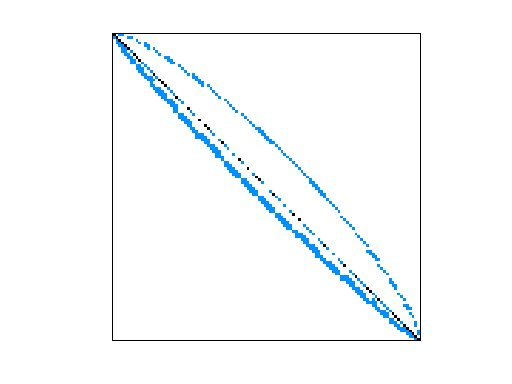
\includegraphics[width=1.1\linewidth]{figures/gre_216a/matrix.png}
    \caption{}		
  \end{subfigure}
  \quad
  \begin{subfigure}[t]{0.45\linewidth}
    \centering
    \includegraphics[width=1.15\linewidth]{figures/gre_216a/figure\thegrecounter.pdf}\stepcounter{grecounter}
    \caption{}
  \end{subfigure}
  \caption{Matrix HB/gre_216a and its GMRES convergence history.}\label{fig:gre_216a}
\end{figure}
\begin{figure}[!ht]
  \centering
  \begin{subfigure}[t]{0.45\linewidth}
    \centering
    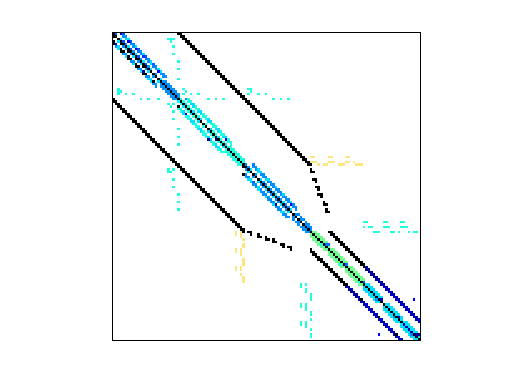
\includegraphics[width=1.1\linewidth]{figures/pores_2/matrix.png}
    \caption{}	
  \end{subfigure}
  \quad
  \begin{subfigure}[t]{0.45\linewidth}
    \centering
    \includegraphics[width=1.15\linewidth]{figures/pores_2/right/figure\theporescounter.pdf}\stepcounter{porescounter}

    \caption{}
  \end{subfigure}
  \caption{Matrix HB/pores_2 and its preconditioned-GMRES convergence history.}\label{fig:pores_2}	
\end{figure}





\begin{table}[ht]
  \caption{Matrices used} % title of Table
  \centering % used for centering table
  \begin{tabular}{c c c c} % centered columns (4 columns)
    \hline\hline %inserts double horizontal lines
    Name & Size (n)& Non-Zeros (\%) & type \\ [0.5ex] % inserts table
    % heading
    \hline % inserts single horizontal line
    HB/arc130 & $130$ & 0.061 & real unsymmetric \\ % inserting body of the table
    Bai/lop163 & $163$ & 0.035 & real unsymmetric  \\
    HB/mcca & $183$ & 0.082 & real unsymmetric  \\
    Rajat/rajat14 & $180$ & 0.046 & real unsymmetric  \\
    HB/fs_183_1 & $183$ & 0.030 & real unsymmetric  \\
    Bai/rdb200 & $200$ & 0.028 & real unsymmetric  \\
    JGD_Trefethen/Trefethen_200 & $200$ & 0.072 & real unsymmetric  \\
    HB/impcol_a & $207$ & 0.013 & real unsymmetric  \\
    HB/gre_216a & $216$ & 0.017 & real unsymmetric  \\
    HB/steam1 & $240$ & 0.039 & real unsymmetric  \\ [1ex] % [1ex] adds vertical space
    \hline %inserts single line
  \end{tabular}
  \label{table:nonlin} % is used to refer this table in the text
\end{table}



\subsection{Representation of executions}
Since an execution can be represented in many different ways, we propose in the following two visualizations enabling the key information to be displayed. The main purpose of the GMRES algorithm is to reduce the residual norm to the target accuracy, hence we use its convergence history, referring to the residual norm evolution through the iterations. Figure~\ref{fig:gre_216a_conv_hist} plots the convergence history of a GMRES execution on gre_216a, disrupted by a transient fault, as well as the same non-faulty execution for reference. We first observe that the true residual in the non-faulty execution (dashed blue curve) converges in $150$ iterations since it reaches the target accuracy ($\varepsilon = 10^{-10}$) at iteration 150. Then, the computed residual in the faulty execution also converges but much later (around iteration 195). On the contrary, the true residual in the faulty execution never reaches the target accuracy, as it remains greater than $10^{-7}$, so according to the definition, the faulty execution fails to converge. The fault (occurring at iteration 70) is responsible for this failure, and it can also be seen that after the fault occurrence, the residual norm decreases more slowly in the faulty execution, which imply more iterations than the reference and potentially a delayed solution (correct or incorrect).

The second way used to represent an execution is simply by its outcome. For instance, Table~\ref{table:outcomes} represents a set of outcomes used later in this report.






\begin{figure}[!ht]
  \centering
  \includegraphics[width=0.7\linewidth]{figures/gre_216a/figure\thegrecounter.pdf}\stepcounter{grecounter}

    \caption{Convergence history of a GMRES execution on gre_216a disrupted by a transient fault (red circle). The Y axis corresponds to the residual norm, and the X axis is the iteration where it was measured. The dashed green line corresponds to the true residual norm in the reference non-faulty execution, the full green line is the true residual norm in the faulty execution (the fault parameters are displayed at the bottom left hand corner) and the blue line is the computed residual norm in the faulty execution.}\label{fig:gre_216a_conv_hist}
  \end{figure}



  \begin{table}[h]
    \centering
    \caption{Color used for each test outcome.}
    \label{table:outcomes}
    \begin{tabular}{|c|}
      \hline
      Outcome  \tabularnewline
      \hline
      \color[RGB]{50, 150, 50}{\textbf{Convergence without delay}} \\
      \color{blue}{\textbf{Convergence with delay}} \\
      \color{red}{\textbf{No convergence}} \\

      \hline
    \end{tabular}
  \end{table}


  
% \subsection{Fault, failure and error}
% The following taxonomy is used~\cite{fault_taxonomy} :
% \begin{itemize}
% \item A fault is 
% \item An error is
% \item A failure is 
% \end{itemize}
% Transient faults, \\
% Soft error, \\
% \subsection*{Notations}
% When a quantity relates to a faulty execution, a '$\sim$' is added on top of the symbol used for the same quantity in the non-faulty execution.

% \newpage


% \begin{algorithm}
%   \caption{Faulty product $z \leftarrow A \cdot v$}\label{alg:faulty_product}
%   \begin{algorithmic}[1]
%     \For {$i = 0,..., n-1$}
%     \State $z_i \gets 0$
%     \For {$k = 0,..., n-1$}
%     \If {$A_{i, k} \neq 0 \text{ and } v_k \neq 0$}
%     \State \text{a bit flip may happen during the following operations}
%     \State $reg_1 \xleftarrow{vulnerable} A_{i, k}$
%     \State $reg_2 \xleftarrow{vulnerable} v_k$ 
%     \State $reg_3 \xleftarrow{vulnerable} reg_1 \cdot reg_2$
%     \State $z_i \gets z_i + reg_3$
%     \EndIf
%     \EndFor
%     \EndFor
%   \end{algorithmic}
% \end{algorithm}

\section{Fault impact analysis}\label{sec:analysis}
In this section, the impact of faults on the convergence of GMRES executions is studied. The impact is first observed both qualitatively and quantitatively on a few cases and according to the previously described experimental setup, and is then analysed from a more theoretical point of view.
\subsection{Empirical study of executions disrupted by faults and fault parameters influence on the convergence}\label{sec:empirical}
To visualize the impact of soft-errors on the convergence, several faults with varying parameters are injected into GMRES executions. In Appendix~\ref{apd:parameters}, each parameter influence is illustrated by three convergence histories for both full-GMRES and right-preconditioned-GMRES. Instinctively, bit-flips on the most significant bits are more likely to prevent the execution from converging than bit-flips on the least significant bits, since they introduce larger error. Less intuitively, faults occurring at the early stage of the execution of a larger impact than faults occurring toward the end. In the following, we reduce the parameter space to those two parameters, since the fault location and the register disrupted seem to have a smaller and rather unpredictable impact on the convergence.
% To visualize the impact of soft-errors on the convergence, different faults are injected into GMRES executions. First qualitative results on a few cases are given to illustrate in detail each fault parameter, and then, quantitative experiments using several matrices are performed to evaluate more extensively the fault effects on GMRES executions. 


%   \subsubsection{Qualitative results and fault parameters influence}
  % To visualize the influence of each fault parameter, the convergence history of 3 disrupted GMRES executions over the same matrices (HB/gre_216a for GMRES and HB/pores_2 for preconditioned-GMRES) are plotted for each one of the 4 fault parameters (bit flipped, iteration, register and location) while the others are fixed. Since both variants of preconditioned-GMRES give similar results, only the right-preconditioned-GMRES ones are displayed.

  % In Figure \ref{fig:conv_hist_bit} all parameters but the bit flipped are fixed. It can be observed that bit-flips on the most significant bits have a stronger impact on the convergence than bit-flips on the least significant bits: in Figure~\ref{fig:gre_216a_conv_hist_bit_0}, the bit flipped is one of the register's least significant bit (bit 60) and the fault does not prevent the convergence. In Figure~\ref{fig:gre_216a_conv_hist_bit_1}, the $40^{th}$ bit is flipped and the convergence is delayed by a dozen iterations. In Figure \ref{fig:gre_216a_conv_hist_bit_2} the $20^{th}$ bit is flipped and the execution never converges to the target accuracy.
  % Intuitively, bit flips on the most significant bits introduce bigger errors and are more likely to disrupt the convergence than bit flips on the least significant bits.





  % \begin{figure}[!ht]
  %   \centering
    
  %   \begin{minipage}[b]{0.45\linewidth}
  %     \centering
  %     \textbf{GMRES} executions on \textbf{gre_216a} 
  %   \end{minipage}
  %   \quad
  %   \begin{minipage}{0.45\linewidth}
  %     \centering
  %     \textbf{preconditioned-GMRES} on \textbf{pores_2}
  %   \end{minipage}\\


  %   \begin{minipage}[b]{0.48\linewidth}
  %     \begin{subfigure}[t]{\linewidth}
  %       \centering
  %       \includegraphics[width=1.15\linewidth]{figures/gre_216a/figure\thegrecounter.pdf}\stepcounter{grecounter}
  %       \caption{bit 0}\label{fig:gre_216a_conv_hist_bit_0}		
  %     \end{subfigure}
  %     \quad
  %     \begin{subfigure}[t]{\linewidth}
  %       \centering
  %       \includegraphics[width=1.15\linewidth]{figures/gre_216a/figure\thegrecounter.pdf}\stepcounter{grecounter}
  %       \caption{bit 25}\label{fig:gre_216a_conv_hist_bit_1}
  %     \end{subfigure}
  %     \quad
  %     \begin{subfigure}[t]{\linewidth}
  %       \centering
  %       \includegraphics[width=1.15\linewidth]{figures/gre_216a/figure\thegrecounter.pdf}\stepcounter{grecounter}
  %       \caption{bit 50}\label{fig:gre_216a_conv_hist_bit_2}
  %     \end{subfigure}
  %   \end{minipage}
  %   \quad
  %   \begin{minipage}[b]{0.48\linewidth}
  %     \begin{subfigure}[t]{\linewidth}
  %       \centering
  %       \includegraphics[width=1.15\linewidth]{figures/pores_2/right/figure\theporescounter.pdf}\stepcounter{porescounter}
  %       \caption{bit 0}\label{fig:pores_2_conv_hist_bit_0}		
  %     \end{subfigure}
  %     \quad
  %     \begin{subfigure}[t]{\linewidth}
  %       \centering
  %       \includegraphics[width=1.15\linewidth]{figures/pores_2/right/figure\theporescounter.pdf}\stepcounter{porescounter}
  %       \caption{bit 25}\label{fig:pores_2_conv_hist_bit_1}
  %     \end{subfigure}
  %     \quad
  %     \begin{subfigure}[t]{\linewidth}
  %       \centering
  %       \includegraphics[width=1.15\linewidth]{figures/pores_2/right/figure\theporescounter.pdf}\stepcounter{porescounter}
  %       \caption{bit 50}\label{fig:pores_2_conv_hist_bit_2}
  %     \end{subfigure}

      
  %   \end{minipage}
  %   \caption{Convergence history of 3 GMRES executions on gre_216a and 3 preconditioned-GMRES executions on pores_2, disrupted by a transient fault. In the execution \ref{fig:gre_216a_conv_hist_bit_0}, the fault (\textbf{bit 0}) disrupts the convergence, in \ref{fig:gre_216a_conv_hist_bit_1}, the fault (\textbf{bit 25}) delays it, and in \ref{fig:gre_216a_conv_hist_bit_2}, the fault (\textbf{bit 50}) has no effect on the convergence. In both cases, bit-flips on the most significant bits have a larger impact than bit-flips on the least significant bits. }\label{fig:conv_hist_bit}
  % \end{figure}



  % In Figure~\ref{fig:conv_hist_iteration}, all parameters but the iteration when the fault occurs are fixed. It can be observed in both GMRES and preconditioned-GMRES that the sooner the fault occurred, the bigger the impact on convergence seems to be: in Figure \ref{fig:gre_216a_conv_hist_iteration_0}, the fault occurred on the $1^{st}$ iteration and the execution did not converge, in Figure \ref{fig:gre_216a_conv_hist_iteration_1}, the fault occurs on the $61^{st}$ iteration and the convergence is delayed, and in Figure \ref{fig:gre_216a_conv_hist_iteration_2} the fault occurs on the $121^{st}$ iteration and the execution converges to the target accuracy.
  % This observations complies with the intuition that the first iterations are responsible for the main part of the solution, while latter ones are responsible for its refinement, hence faults are more likely to be critical when occurring at the early stages of the execution than towards the end.





  % \begin{figure}[!ht]
  %   \centering
    
  %   \begin{minipage}[b]{0.45\linewidth}
  %     \centering
  %     \textbf{GMRES} executions on \textbf{gre_216a} 
  %   \end{minipage}
  %   \quad
  %   \begin{minipage}{0.45\linewidth}
  %     \centering
  %     \textbf{preconditioned-GMRES} on \textbf{pores_2}
  %   \end{minipage}\\


  %   \begin{minipage}[b]{0.48\linewidth}
  %     \begin{subfigure}[t]{\linewidth}
  %       \centering
  %       \includegraphics[width=1.15\linewidth]{figures/gre_216a/figure\thegrecounter.pdf}\stepcounter{grecounter}
  %       \caption{iteration 10}\label{fig:gre_216a_conv_hist_iteration_0}		
  %     \end{subfigure}
  %     \quad
  %     \begin{subfigure}[t]{\linewidth}
  %       \centering
  %       \includegraphics[width=1.15\linewidth]{figures/gre_216a/figure\thegrecounter.pdf}\stepcounter{grecounter})
  %       \caption{iteration 60}\label{fig:gre_216a_conv_hist_iteration_1}
  %     \end{subfigure}
  %     \quad
  %     \begin{subfigure}[t]{\linewidth}
  %       \centering
  %       \includegraphics[width=1.15\linewidth]{figures/gre_216a/figure\thegrecounter.pdf}\stepcounter{grecounter})
  %       \caption{iteration 110}\label{fig:gre_216a_conv_hist_iteration_2}
  %     \end{subfigure}
  %   \end{minipage}
  %   \quad
  %   \begin{minipage}[b]{0.48\linewidth}
  %     \begin{subfigure}[t]{\linewidth}
  %       \centering
  %       \includegraphics[width=1.15\linewidth]{figures/pores_2/right/figure\theporescounter.pdf}\stepcounter{porescounter}
  %       \caption{iteration 5}\label{fig:pores_2_conv_hist_iteration_0}		
  %     \end{subfigure}
  %     \quad
  %     \begin{subfigure}[t]{\linewidth}
  %       \centering
  %       \includegraphics[width=1.15\linewidth]{figures/pores_2/right/figure\theporescounter.pdf}\stepcounter{porescounter}
  %       \caption{iteration 10}\label{fig:pores_2_conv_hist_iteration_1}
  %     \end{subfigure}
  %     \quad
  %     \begin{subfigure}[t]{\linewidth}
  %       \centering
  %       \includegraphics[width=1.15\linewidth]{figures/pores_2/right/figure\theporescounter.pdf}\stepcounter{porescounter}
  %       \caption{iteration 15}\label{fig:pores_2_conv_hist_iteration_2}
  %     \end{subfigure}

      
  %   \end{minipage}
  %   \caption{Convergence history of 3 GMRES executions on gre_216a and 3 preconditioned-GMRES executions on pores_2, disrupted by a transient fault. In the execution \ref{fig:gre_216a_conv_hist_iteration_0}, the fault (\textbf{iteration 10}) disrupts the convergence, in \ref{fig:gre_216a_conv_hist_iteration_1}, the fault (\textbf{iteration 60}) delays it, and in \ref{fig:gre_216a_conv_hist_iteration_2}, the fault (\textbf{iteration 110}) has no effect on the convergence. In both cases, the fault impact decreases as the iteration when it is injected increases.}\label{fig:conv_hist_iteration}
  % \end{figure}




  % The remaining fault parameters (register and location) do not appear to have any significant impact on the convergence, even though inputs can be constructed to contradict this observation. Figure \ref{fig:conv_hist_register}, representing the convergence history of 3 GMRES executions and 3 preconditioned-GMRES disrupted by a bit-flip on $reg_1$, $reg_2$ and $reg_3$, and Figure \ref{fig:conv_hist_location}, representing the convergence history of 3 GMRES executions and 3 preconditioned-GMRES disrupted by a bit-flip on three different locations, present similar behaviors in terms of convergence history.



  % \begin{figure}[!ht]
  %   \centering
    
  %   \begin{minipage}[b]{0.45\linewidth}
  %     \centering
  %     \textbf{GMRES} executions on \textbf{gre_216a} 
  %   \end{minipage}
  %   \quad
  %   \begin{minipage}{0.45\linewidth}
  %     \centering
  %     \textbf{preconditioned-GMRES} on \textbf{pores_2}
  %   \end{minipage}\\


  %   \begin{minipage}[b]{0.48\linewidth}
  %     \begin{subfigure}[t]{\linewidth}
  %       \centering
  %       \includegraphics[width=1.15\linewidth]{figures/gre_216a/figure\thegrecounter.pdf}\stepcounter{grecounter})
  %       \caption{$reg_1$}\label{fig:gre_216a_conv_hist_register_0}		
  %     \end{subfigure}
  %     \quad
  %     \begin{subfigure}[t]{\linewidth}
  %       \centering
  %       \includegraphics[width=1.15\linewidth]{figures/gre_216a/figure\thegrecounter.pdf}\stepcounter{grecounter})
  %       \caption{$reg_2$}\label{fig:gre_216a_conv_hist_register_1}
  %     \end{subfigure}
  %     \quad
  %     \begin{subfigure}[t]{\linewidth}
  %       \centering
  %       \includegraphics[width=1.15\linewidth]{figures/gre_216a/figure\thegrecounter.pdf}\stepcounter{grecounter})
  %       \caption{$reg_3$}\label{fig:gre_216a_conv_hist_register_2}
  %     \end{subfigure}
  %   \end{minipage}
  %   \quad
  %   \begin{minipage}[b]{0.48\linewidth}
  %     \begin{subfigure}[t]{\linewidth}
  %       \centering
  %       \includegraphics[width=1.15\linewidth]{figures/pores_2/right/figure\theporescounter.pdf}\stepcounter{porescounter}
  %       \caption{$reg_1$}\label{fig:pores_2_conv_hist_register_0}		
  %     \end{subfigure}
  %     \quad
  %     \begin{subfigure}[t]{\linewidth}
  %       \centering
  %       \includegraphics[width=1.15\linewidth]{figures/pores_2/right/figure\theporescounter.pdf}\stepcounter{porescounter}
  %       \caption{$reg_2$}\label{fig:pores_2_conv_hist_register_1}
  %     \end{subfigure}
  %     \quad
  %     \begin{subfigure}[t]{\linewidth}
  %       \centering
  %       \includegraphics[width=1.15\linewidth]{figures/pores_2/right/figure\theporescounter.pdf}\stepcounter{porescounter}
  %       \caption{$reg_3$}\label{fig:pores_2_conv_hist_register_2}
  %     \end{subfigure}

      
  %   \end{minipage}
  %   \caption{Convergence history of 3 GMRES executions on gre_216a and 3 preconditioned-GMRES executions on pores_2, disrupted by a transient fault. In all the executions, the faults (occurring in $reg_1$, $reg_2$ and $reg_3$) seem to have the same impact.}\label{fig:conv_hist_register}
  % \end{figure}







  % \begin{figure}[!ht]
  %   \centering
    
  %   \begin{minipage}[b]{0.45\linewidth}
  %     \centering
  %     \textbf{GMRES} executions on \textbf{gre_216a} 
  %   \end{minipage}
  %   \quad
  %   \begin{minipage}{0.45\linewidth}
  %     \centering
  %     \textbf{preconditioned-GMRES} on \textbf{pores_2}
  %   \end{minipage}\\


  %   \begin{minipage}[b]{0.48\linewidth}
  %     \begin{subfigure}[t]{\linewidth}
  %       \centering
  %       \includegraphics[width=1.15\linewidth]{figures/gre_216a/figure\thegrecounter.pdf}\stepcounter{grecounter})
  %       \caption{}\label{fig:gre_216a_conv_hist_location_0}		
  %     \end{subfigure}
  %     \quad
  %     \begin{subfigure}[t]{\linewidth}
  %       \centering
  %       \includegraphics[width=1.15\linewidth]{figures/gre_216a/figure\thegrecounter.pdf}\stepcounter{grecounter})
  %       \caption{}\label{fig:gre_216a_conv_hist_location_1}
  %     \end{subfigure}
  %     \quad
  %     \begin{subfigure}[t]{\linewidth}
  %       \centering
  %       \includegraphics[width=1.15\linewidth]{figures/gre_216a/figure\thegrecounter.pdf}\stepcounter{grecounter})
  %       \caption{}\label{fig:gre_216a_conv_hist_location_2}
  %     \end{subfigure}
  %   \end{minipage}
  %   \quad
  %   \begin{minipage}[b]{0.48\linewidth}
  %     \begin{subfigure}[t]{\linewidth}
  %       \centering
  %       \includegraphics[width=1.15\linewidth]{figures/pores_2/right/figure\theporescounter.pdf}\stepcounter{porescounter}
  %       \caption{}\label{fig:pores_2_conv_hist_location_0}		
  %     \end{subfigure}
  %     \quad
  %     \begin{subfigure}[t]{\linewidth}
  %       \centering
  %       \includegraphics[width=1.15\linewidth]{figures/pores_2/right/figure\theporescounter.pdf}\stepcounter{porescounter}
  %       \caption{}\label{fig:pores_2_conv_hist_location_1}
  %     \end{subfigure}
  %     \quad
  %     \begin{subfigure}[t]{\linewidth}
  %       \centering
  %       \includegraphics[width=1.15\linewidth]{figures/pores_2/right/figure\theporescounter.pdf}\stepcounter{porescounter}
  %       \caption{}\label{fig:pores_2_conv_hist_location_2}
  %     \end{subfigure}

      
  %   \end{minipage}
  %   \caption{Convergence history of 3 GMRES executions on gre_216a and 3 preconditioned-GMRES executions on pores_2, disrupted by a transient fault. In all the executions, the faults (occurring in random locations) seem to have the same impact.}\label{fig:conv_hist_location}
  % \end{figure}

  % In summary, only the bit and the iteration where the bitflip occurs seems to have a significant impact on the convergence. For this reason, the fault parameter space to cover is reduced to those two parameters, simplifying the quantitative results presented in the next section.
  
  %\subsubsection{Quantitative results}

  %To illustrate the previous observations,
Figure~\ref{fig:bit_iteration} presents the convergence outcome of several faulty-executions - one for each couple (iteration fault $\times$ bit flipped) while the other parameters are chosen randomly - for GMRES on HB/gre_216a and right-preconditioned-GMRES on HB/pores_2. Some faults have no effect on the convergence (in green), some may only delay it (blue), and others may prevent the execution from converging to the target accuracy (red). As observed in Appendix~\ref{apd:parameters}, faults involving the most significant bits of the registers or happening soon in the execution are more likely to cause a failure than faults involving the least significant bits or happening late in the execution.






  \begin{figure}[!ht] 
    \hspace{3ex}
    \begin{minipage}[b]{0.5\linewidth}
      \centering
      \textbf{GMRES} executions on \textbf{gre_216a} 
    \end{minipage}
    \quad
    \begin{minipage}{0.5\linewidth}
      \centering
      \textbf{preconditioned-GMRES} on \textbf{pores_2}
    \end{minipage}\\

    \begin{subfigure}[b]{0.5\linewidth}
      \centering
      \includegraphics[width=1.15\linewidth]{figures/gre_216a/figure\thegrecounter.pdf}\stepcounter{grecounter})
      \caption{$\varepsilon = 10^{-5}$}
      \label{fig:gre_216a_bit_iteration_0}	
    \end{subfigure}%% 
    \hspace{4ex}
    \begin{subfigure}[b]{0.5\linewidth}
      \centering
      \includegraphics[width=1.15\linewidth]{figures/pores_2/right/figure\theporescounter.pdf}\stepcounter{porescounter}
      \caption{$\varepsilon = 10^{-5}$}
      \label{fig:pores_2_bit_iteration_0}	
    \end{subfigure} 

    \begin{subfigure}[b]{0.5\linewidth}
      \centering
      \includegraphics[width=1.15\linewidth]{figures/gre_216a/figure\thegrecounter.pdf}\stepcounter{grecounter})
      \caption{$\varepsilon = 10^{-10}$}
      \label{fig:gre_216a_bit_iteration_1}	
    \end{subfigure}%%
    \hspace{4ex}
    \begin{subfigure}[b]{0.5\linewidth}
      \centering
      \includegraphics[width=1.15\linewidth]{figures/pores_2/right/figure\theporescounter.pdf}\stepcounter{porescounter}
      \caption{$\varepsilon = 10^{-10}$}
      \label{fig:pores_2_bit_iteration_1}	
    \end{subfigure} 
    \caption{Diagram of executions disrupted by a fault. Each dot represents an execution of GMRES on HB/gre_216a (figures \ref{fig:gre_216a_bit_iteration_0} and \ref{fig:gre_216a_bit_iteration_1}) or preconditioned-GMRES on HB/pores_2 (figures \ref{fig:pores_2_bit_iteration_0} and \ref{fig:pores_2_bit_iteration_1}), its abscissa is the bit where the fault occurred, its ordinate is the moment in the execution when the fault has been injected and its color represents whether the execution has converged or not (green: no delay, red: no convergence, blue: delayed convergence).}
    \label{fig:bit_iteration}
  \end{figure}





  As shown in Figure~\ref{fig:matrices_bit_iteration}, the behavior of faulty GMRES is very similar for all the selected matrices: the left-hand side of the graphs corresponding to executions disrupted by bit-flips of the most significant bit mostly fail to converge, except for the latest iterations, while the right-hand side of the graphs corresponding to executions where the least significant bits are flipped usually converges. %TODO: refaire les graphs (l�gende + preconditioned-gmres)




  \begin{figure}[!ht] 
    \hspace{3ex}


    \begin{subfigure}[b]{0.5\linewidth}
      \centering
      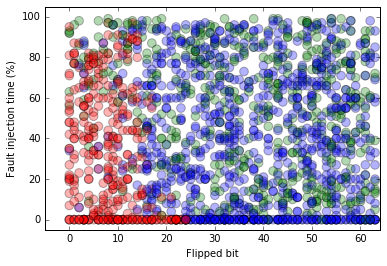
\includegraphics[width=\linewidth]{figures/bit_iteration_0.png} %TODO
      \caption{$\varepsilon = 10^{-5}$}
      \label{fig:bit_iteration_0}	
    \end{subfigure}%% 
    \hspace{4ex}
    \begin{subfigure}[b]{0.5\linewidth}
      \centering
      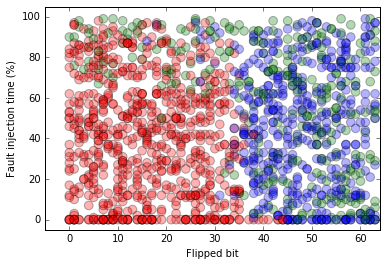
\includegraphics[width=\linewidth]{figures/bit_iteration_1.png} %TODO
      \caption{$\varepsilon = 10^{-10}$}
      \label{fig:bit_iteration_1}	
    \end{subfigure} 

    \caption{Diagrams of GMRES executions disrupted by a fault. Each dot represents an execution on any matrix of the dataset, its abscissa is the bit where the fault occurred, its ordinate is the moment in the execution when the fault has been injected and its color represents whether the execution has converged or not (green: no delay, red: no convergence, blue: delayed convergence).}
    \label{fig:matrices_bit_iteration}
  \end{figure}








%  \newpage

  % From \cite{DBLP:journals/siamsc/GiraudGL07} : 
  % \begin{equation}\label{eqn:delta}
  %   \text{delta = } \|\widetilde{r_l} - \widetilde{r_l}\textprime \| = ||y_{l, k}(z_{k+1} - z_{k+1})\| 
  % \end{equation}


  \subsection{Analytical study of the fault impact on the convergence}\label{sec:analytical}
  
  In the previous experiments, we showed that a transient fault may have a significant impact on the convergence of an execution. In the following, an analysis is proposed to evaluate this impact using the theory of inexact GMRES, in order to intent to predict the convergence behavior in~\ref{sec:prediction}.


  % \subsubsection{Error propagation}\label{sec:propagation}
  % At the fault iteration $i=f$, some variables become corrupted as illustrated in Figure \ref{fig:error_propagation}. At first, only one value in the vector $w = A \cdot v_f$ is erroneous, but this error gets spread out in the orthonormalization process (modified Gram-Schmidt), generating a wrong new arnoldi vector $v_{f+1}$ as well as a wrong last column in the Hessenberg matrix $H_{f+1}$, resulting in a different Krylov space and potentially leading to an incorrect solution. Moreover, the erroneous Arnoldi basis ($V_{f+1}$) and Hessenberg matrix ($H_{f+1}$) are used in the next iterations, which may increase the deviation from the correct execution even further. 
  % \begin{figure}[!ht]
  %   \centering
  %   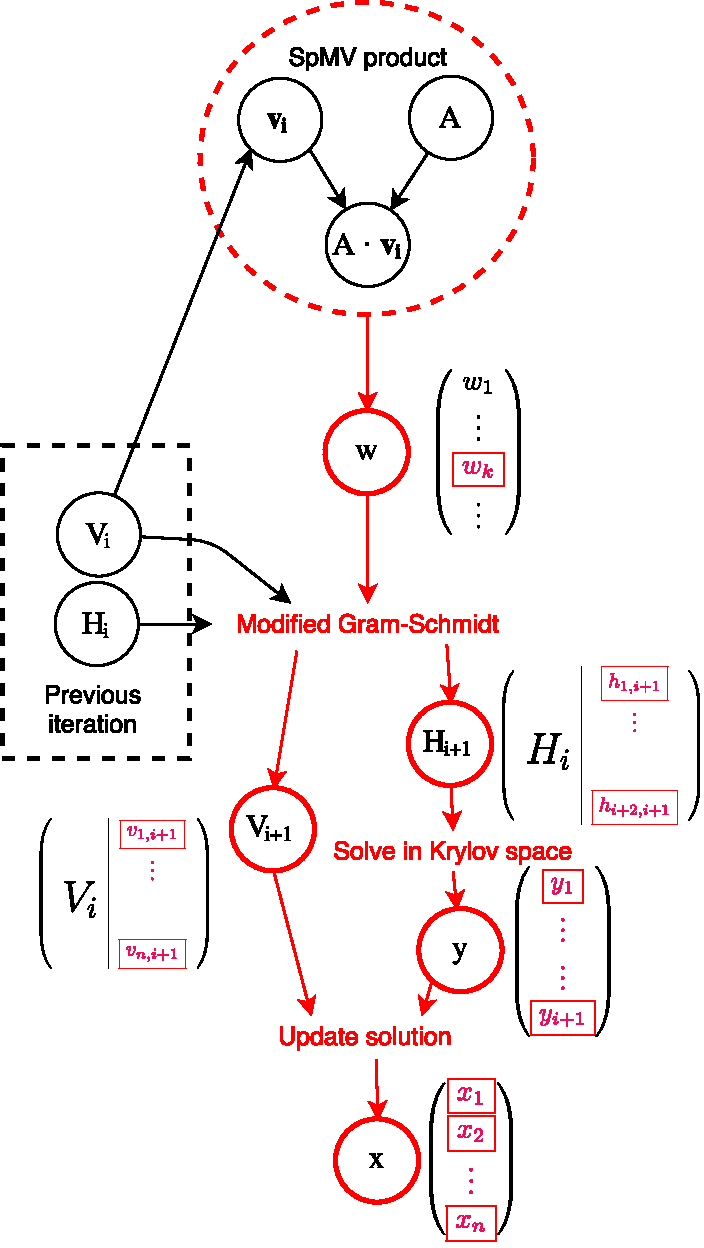
\includegraphics[scale=0.4]{figures/error_propagation.pdf}
  %   \caption{Error (red) propagation at the fault iteration.}\label{fig:error_propagation}
  % \end{figure}

  \subsubsection{Error quantification}\label{sec:quantify}
  Because the sequence of least-square problems solved along the iteration are nested; that is at iteration $i$ 
  the leading part of $H_{i+1}$ is $H_i$ as well as for the right-hand sides; we know that independently of the possible occurrence of a fault during the execution, GMRES always reduces the computed residual norm down to the machine accuracy, as long as it is given enough iterations to do so. However, a fault may introduce a large residual deviation between the computed residual and the true residual (i.e., $\|\widetilde{r}_{\ell} - \widetilde{r}_{\ell}\textprime \|$ becomes large), which may prevent the latter one from reaching the target accuracy. Since $ \|\widetilde{r}_{\ell}\| \geq \|\widetilde{r}_{\ell} - \widetilde{r}_{\ell}\textprime \| - \| \widetilde{r}_{\ell}\textprime \|$ and $\|\widetilde{r}_\ell\textprime \| \rightarrow 0$, we obtain that $\|\widetilde{r}_{\ell}\| \rightarrow \|\widetilde{r}_{\ell} - \widetilde{r}_\ell\textprime \|$, so if the error remains greater than the target accuracy $\varepsilon$, the execution will not converge. The error measured at iteration $\ell$ is called the residual gap at iteration $\ell$, denoted $\delta(\ell)$.
  We illustrate in Figure \ref{fig:conv_hist_true_delta} the effect of a soft-error on the norm of the residuals and the measured residual gap $\|\widetilde{r}_{i} - \widetilde{r}_{i}\textprime \|$.
  Before the fault, the residual gap is close to the machine accuracy. After the fault and until the end of the execution, the residual gap fluctuates and gets closer to the true residual norm (green line) as the computed residual norm (blue line) converges to the machine accuracy.
  The dashed green line shows the non-faulty execution residuals, to illustrate the delay induced by the error in the convergence.
  The residual gap provides a good quantification of the fault impact, however it does not explain nor quantifies how much the convergence is delayed (when the convergence occurs).




  \begin{figure}[!ht]
    \centering
    \begin{subfigure}[t]{0.45\linewidth}
      \centering
      \includegraphics[width=1.15\linewidth]{figures/gre_216a/figure\thegrecounter.pdf}\stepcounter{grecounter})
      \caption{GMRES on gre_216a}\label{fig:gre_216a_conv_hist_true_delta}		
    \end{subfigure}
    \quad
    \begin{subfigure}[t]{0.45\linewidth}
      \centering
      \includegraphics[width=1.15\linewidth]{figures/pores_2/right/figure\theporescounter.pdf}\stepcounter{porescounter}
      \caption{preconditioned-GMRES on pores_2, }\label{fig:pores_2_conv_hist_true_delta}
    \end{subfigure}
    \caption{Two convergence histories disrupted by a fault. The light blue line represents the residual gap evolution in the faulty executions:GMRES on gre_216a in \ref{fig:gre_216a_conv_hist_true_delta} and precondition-GMRES  on pores_2 in \ref{fig:pores_2_conv_hist_true_delta}.}
  \end{figure}\label{conv_hist_true_delta}



  % TODO y-axis error

  In~\cite{sisz:03}, the authors provide a general framework for the understanding of inexact Krylov subspaces, generated by inexact matrix vector products that arise naturally in many scientific applications. In particular, they analyze the residual norm deviation assuming that a perturbation $E_i$ is applied to the SpMV product at each
  iteration $i$. 
  \begin{equation}\label{inexact_krylov}
    \widetilde{r}_\ell = \widetilde{r}_\ell\textprime + \widetilde{y_\ell} \cdot \sum_{i=1}^{\ell}{E_i \cdot v_i}\text{.}
  \end{equation}

  We can use this analysis in a somehow simpler situation where a transient fault is considered as a perturbation $E_f$ that only occurs once at the $f^{th}$ iteration, specializing the results in ~\cite{sisz:03} to be applicable in our model.
  \begin{equation}\label{inexact_krylov_adapted}
    \| \widetilde{r}_\ell - \widetilde{r}_\ell\textprime \| =  \| \widetilde{y_\ell} \cdot E_f \cdot v_f \|\text{.}
  \end{equation}

  This enables us to get the following equation that links the residual gap to $\widetilde{y}_{\ell, f}$ and to the error introduced by the fault $\|E_f \cdot v_f\| = \|A \cdot {v}_{f} - \widetilde{A} \cdot v_{f}\| = \|{w}_{f+1} - \widetilde{w}_{f+1}\|$ :
  \begin{equation}\label{eqn:delta}
    \delta(\ell) = \|\widetilde{r}_{\ell} - \widetilde{r}_{\ell}\textprime \| = |\widetilde{y}_{{\ell}, f}|\cdot \|{w}_{f+1} - \widetilde{w}_{f+1}\|\text{.}
  \end{equation}
  where  $w_{f+1}$ is the $f+1^{th}$ Arnoldi vector before orthonormalization and $\widetilde{y}_{\ell, f}$ is the $f^{th}$ component of the $\ell^{th}$ least square problem solution $\widetilde{y}_\ell=\argmin_{\mathbf{y_{}}}\|\beta e_1 - H_{\ell} \mathbf{y_{}}\|$. In the following, the quantity $|\widetilde{y}_{{i}, f}|\cdot \|{w}_{f+1} - \widetilde{w}_{f+1}\|$ is called the computed residual gap at iteration $i$, in constrast with the measured residual gap at iteration i $\|\widetilde{r}_{i} - \widetilde{r}_{i}\textprime \|$. These quantities are equal when $i = \ell$.


  \begin{figure}[!ht]
    \centering
    \begin{subfigure}[t]{0.45\linewidth}
      \centering
      \includegraphics[width=1.15\linewidth]{figures/gre_216a/figure\thegrecounter.pdf}\stepcounter{grecounter})
      \caption{GMRES on gre_216a}\label{fig:gre_216a_conv_hist_delta}		
    \end{subfigure}
    \quad
    \begin{subfigure}[t]{0.45\linewidth}
      \centering
      \includegraphics[width=1.15\linewidth]{figures/pores_2/right/figure\theporescounter.pdf}\stepcounter{porescounter}
      \caption{preconditioned-GMRES on pores_2, }\label{fig:pores_2_conv_hist_delta}
    \end{subfigure}
    \caption{Two convergence histories disrupted by a fault. The light blue and purple lines represent the measured residual gap ($\|\widetilde{r}_{i} - \widetilde{r}_{i}\textprime \|$) and the computed residual gap ($|\widetilde{y}_{{i}, f}|\cdot \|{w}_{f+1} - \widetilde{w}_{f+1}\|$) evolutions in the faulty executions:GMRES on gre_216a in \ref{fig:gre_216a_conv_hist_delta} and precondition-GMRES  on pores_2 in \ref{fig:pores_2_conv_hist_delta}.}
  \end{figure}

  \subsubsection{Prediction of the fault impact}\label{sec:prediction}
  From Section~\ref{sec:empirical}, we observed that faults may either have a critical impact when preventing the execution from converging, little impact when delaying the convergence, or no impact at all. Ideally, by using the symptoms brought by a fault we should be able to predict its impact.
  Theorem~\ref{theorem} below proposes a possible suited criterion in the form of a threshold on the error $\|{w}_{f+1} - \widetilde{w}_{f+1}\|$ to ensure that a fault is not critical.
  It is based on Equation~\eqref{eqn:delta}, itself relying on the remark that a faulty matrix-vector product caused by a bit-flip can be interpreted as an inexact matrix-vector product in inexact~\cite{sisz:03} or
  relaxed~\cite{DBLP:journals/siamsc/GiraudGL07} GMRES.
  \begin{theorem}\label{theorem}
    Let $0 < c < 1$ and let a GMRES execution using a reduced target accuracy $(1-c) \varepsilon$, terminating in $\ell$ iterations and disrupted by a fault at iteration $f < \ell$. In exact arithmetic, if $\|{w}_{f+1} - \widetilde{w}_{f+1}\| < \tau_c = (c \cdot \varepsilon) / |\widetilde{y}_{\ell, f}|$ then the execution converges to the target accuracy $\varepsilon$.
  \end{theorem}
  \begin{proof}
    The purpose of the $c$ parameter is to bound the true residual norm as a convex combination of the residual deviation norm and the computed residual norm.
    Since the GMRES execution terminates in $\ell$ iterations for the target accuracy $(1 - c) \varepsilon$ $$\|\widetilde{r}\textprime_{\ell}\| \leq (1 - c) \varepsilon \text{.}$$
    Then, using Equation \eqref{eqn:delta} derived from \cite{DBLP:journals/siamsc/GiraudGL07} and the criterion $\|{w}_{f+1} - \widetilde{w}_{f+1}\| < \frac{c \cdot \varepsilon}{|\widetilde{y}_{\ell, f}|}$ :
    \begin{equation}
      % 
      \begin{split}
        \|\widetilde{r}_\ell\| & \leq \|\widetilde{r}_\ell - \widetilde{r}\textprime_\ell \| + \|\widetilde{r}\textprime_\ell\| \\
        &\leq \|y_{\ell, f} (w_{f+1} - \widetilde{w}_{f+1}) \| + \|\widetilde{r}\textprime_\ell\| \\
        &\leq |y_{\ell, f}| \cdot \|{w}_{f+1} - \widetilde{w}_{f+1}\| + \|\widetilde{r}\textprime_\ell\| \\
        &\leq c \cdot \varepsilon + (1 - c) \cdot \varepsilon = \varepsilon \text{.}\\
        % 
      \end{split}
    \end{equation}
    The GMRES execution has converged with the target accuracy $\varepsilon$.
  \end{proof}

  \subsubsection{Numerical experiment}
  In order to verify if Theorem~\ref{theorem} is applicable, even in floating point arithmetic instead of exact arithmetic, the following numerical experiments are performed.
    Let $0 < c < 1$, we can predict if the fault will not disrupt the convergence to $\varepsilon$ using Theorem~\ref{theorem} by lowering the target accuracy of the execution to $(1 - c) \cdot \varepsilon$ and by computing the following expression at the fault iteration f:
  \begin{equation}
    \text{error} = \|{w}_{f+1} - \widetilde{w}_{f+1}\| < \tau_c = (c \cdot \varepsilon) / |\widetilde{y}_{\ell, f}|\text{.}
  \end{equation}\label{scheme_oracle}
  If the error introduced by the fault in lower than the threshold, the execution must converge (and then is predicted to converge) to the target accuracy $\varepsilon$ according to Theorem \ref{theorem}. Note that the reverse is not necessarily true so if the error is greater than the threshold, the execution may or may not converge to the target accuracy (no prediction). Figure~\ref{fig:compared} illustrates this idea. It displays the convergence histories of 4 executions disrupted by a fault. At the fault iteration $f$, the error is compared to the threshold. In the upper plots, the error is lower than the threshold, hence the execution is predicted to converge. On the contrary in the bottom plots, the error is greater than the threshold so no convergence prediction can be made (although in both case the executions happen to converge anyway). For the prediction, the value $c=0.5$ was used.



  \begin{figure}[!ht]
    \centering
    
    \begin{minipage}[b]{0.45\linewidth}
      \centering
      \textbf{GMRES} executions on \textbf{gre_216a} 
    \end{minipage}
    \quad
    \begin{minipage}{0.45\linewidth}
      \centering
      \textbf{preconditioned-GMRES} on \textbf{pores_2}
    \end{minipage}\\


    \begin{minipage}[b]{0.48\linewidth}
      \begin{subfigure}[t]{\linewidth}
        \centering
        \includegraphics[width=1.15\linewidth]{figures/gre_216a/figure\thegrecounter.pdf}\stepcounter{grecounter})
        \caption{Convergence prediction}\label{fig:gre_216a_conv_hist_prediction}		
      \end{subfigure}
      \quad
      \begin{subfigure}[t]{\linewidth}
        \centering
        \includegraphics[width=1.15\linewidth]{figures/gre_216a/figure\thegrecounter.pdf}\stepcounter{grecounter})
        \caption{No prediction}\label{fig:gre_216a_conv_hist_no_prediction}
      \end{subfigure}
    \end{minipage}
    \quad
    \begin{minipage}[b]{0.48\linewidth}
      \begin{subfigure}[t]{\linewidth}
        \centering
        \includegraphics[width=1.15\linewidth]{figures/pores_2/right/figure\theporescounter.pdf}\stepcounter{porescounter}
        \caption{Convergence prediction}\label{fig:pores_2_conv_hist_prediction}		
      \end{subfigure}
      \quad
      \begin{subfigure}[t]{\linewidth}
        \centering
        \includegraphics[width=1.15\linewidth]{figures/pores_2/right/figure\theporescounter.pdf}\stepcounter{porescounter}
        \caption{No prediction}\label{fig:pores_2_conv_hist_no_prediction}
      \end{subfigure}

      
    \end{minipage}
    \caption{Prediction of the convergence in 4 executions disrupted by a fault on gre_216a and pores_2. At the fault iteration $f$, the error is compared to the threshold. In the upper plots, the error is lower than the threshold, hence the execution is predicted to converge. On the contrary in the bottom plots, the error is greater than the threshold so no convergence prediction can be made (although in both case the executions happen to converge anyway). For the prediction, the value $c=0.5$ was used.}\label{fig:compared}
  \end{figure}



  Figure~\ref{fig:prediction} displays the prediction result for several executions, grouped by convergence outcome, and depending on the fault properties (bit flipped and injection time). Every execution that was predicted to converged (green) has indeed converged to the target accuracy (top and middle plots), since no execution that did not converge (bottom plots) has been predicted to. Despite the use of floating point arithmetic instead of exact arithmetic, Theorem~\ref{theorem} still gives the expected results. For the executions that did converge, the prediction is correct for a large part of cases, except for those closer to non-convergence. In particular, the proportion of predicted convergence is lower when the convergence was delayed.
  
  \begin{figure}[!ht]
    \centering
    
    \begin{minipage}[b]{0.45\linewidth}
      \centering
      \textbf{GMRES} executions on \textbf{gre_216a} 
    \end{minipage}
    \quad
    \begin{minipage}{0.45\linewidth}
      \centering
      \textbf{preconditioned-GMRES} on \textbf{pores_2}
    \end{minipage}\\


    \begin{minipage}[b]{0.48\linewidth}
      \begin{subfigure}[t]{\linewidth}
        \centering
        \includegraphics[width=1.15\linewidth]{figures/gre_216a/figure\thegrecounter.pdf}\stepcounter{grecounter})
        \caption{Converged}\label{fig:gre_216a_conv_hist_location_0}		
      \end{subfigure}
      \quad
      \begin{subfigure}[t]{\linewidth}
        \centering
        \includegraphics[width=1.15\linewidth]{figures/gre_216a/figure\thegrecounter.pdf}\stepcounter{grecounter})
        \caption{Delayed}\label{fig:gre_216a_conv_hist_location_1}
      \end{subfigure}
      \quad
      \begin{subfigure}[t]{\linewidth}
        \centering
        \includegraphics[width=1.15\linewidth]{figures/gre_216a/figure\thegrecounter.pdf}\stepcounter{grecounter})
        \caption{Not converged}\label{fig:gre_216a_conv_hist_location_2}
      \end{subfigure}
    \end{minipage}
    \quad
    \begin{minipage}[b]{0.48\linewidth}
      \begin{subfigure}[t]{\linewidth}
        \centering
        \includegraphics[width=1.15\linewidth]{figures/pores_2/right/figure\theporescounter.pdf}\stepcounter{porescounter}
        \caption{Converged}\label{fig:pores_2_conv_hist_location_0}		
      \end{subfigure}
      \quad
      \begin{subfigure}[t]{\linewidth}
        \centering
        \includegraphics[width=1.15\linewidth]{figures/pores_2/right/figure\theporescounter.pdf}\stepcounter{porescounter}
        \caption{Delayed}\label{fig:pores_2_conv_hist_location_1}
      \end{subfigure}
      \quad
      \begin{subfigure}[t]{\linewidth}
        \centering
        \includegraphics[width=1.15\linewidth]{figures/pores_2/right/figure\theporescounter.pdf}\stepcounter{porescounter}
        \caption{Not converged}\label{fig:pores_2_conv_hist_location_2}
      \end{subfigure}
      

      
    \end{minipage}
    \caption{Prediction of the convergence in several executions disrupted by a fault. Each dot corresponds to an execution, its abscissa is the bit flipped, its ordinate is the fault injection time in the execution, and its color represents whether the execution was predicted to converge (green) or no prediction was made (red). The executions are split into 3 plots for each matrix used, one for each convergence outcome (convergence, delayed convergence and no convergence). For the prediction, the value $c=0.5$ was used. Every execution that was predicted to converged did  (Theorem~\ref{theorem}) since all of them are located in the upper 4 plots (convergence or delayed convergence).}\label{fig:prediction}
  \end{figure}



  % Figure~\ref{fig:test_result_oracle} displays the fault detection scheme results (in percentage of executions) for several values of c.
  % First, no critical faults are ignored, which is a direct consequence of Theorem \ref{theorem}: If a fault Second, for low values of $c$, an important part (between 20\% and 35\%) of executions disrupted by a negligible fault detect it anyway (dark gray) as the detection scheme is more sensitive, but it becomes more and more capable of ignoring those when $c$ increases. The rest of the faulty executions (green and light gray) are correctly handled.

  % For more details, the $c=0.5$ cases are plotted in Figure~\ref{fig:test_result_c05}. In each case, all the critical fault are correctly detectedlarge majority of the faulty executions correctly detects the faults. The rare cases of unneeded detection (dark gray) occur at the limit of the convergence and non convergence domain (light gray and green respectively).





  % \begin{figure}[!ht]
  %   \centering

  %   \begin{minipage}[b]{0.45\linewidth}
  %     \centering
  %     \textbf{full-GMRES} executions on \textbf{gre_216a} 
  %   \end{minipage}
  %   \quad
  %   \begin{minipage}{0.45\linewidth}
  %     \centering
  %     \textbf{preconditioned-GMRES} on \textbf{pores_2}
  %   \end{minipage}\\


  %   \begin{minipage}[b]{0.48\linewidth}

  %     \begin{subfigure}[t]{\linewidth}
  %       \centering
  %       \includegraphics[width=1.1\linewidth]{figures/gre_216a/test_result_oracle_0.png}
  %       \caption{$\varepsilon = 10^{-5}$}\label{fig:gre_216a_test_result_oracle_0}	
  %     \end{subfigure}
  %     \quad
  %     \begin{subfigure}[t]{\linewidth}
  %       \centering
  %       \includegraphics[width=1.1\linewidth]{figures/gre_216a/test_result_oracle_1.png}
  %       \caption{$\varepsilon = 10^{-10}$}\label{fig:gre_216a_test_result_oracle_1}	
  %     \end{subfigure}
  %   \end{minipage}
  %   \quad
  %   \begin{minipage}[b]{0.48\linewidth}

  %     \begin{subfigure}[t]{\linewidth}
  %       \centering
  %       \includegraphics[width=1.1\linewidth]{figures/pores_2/test_result_oracle_0.png}
  %       \caption{$\varepsilon = 10^{-5}$}\label{fig:pores_2_test_result_oracle_0}	
  %     \end{subfigure}
  %     \quad
  %     \begin{subfigure}[t]{\linewidth}
  %       \centering
  %       \includegraphics[width=1.1\linewidth]{figures/pores_2/test_result_oracle_1.png}
  %       \caption{$\varepsilon = 10^{-10}$}\label{fig:pores_2_test_result_oracle_1}	
  %     \end{subfigure}

  %   \end{minipage}
  %   \caption{Diagrams representing the test outcome proportion for several values of c. To compute them, faulty executions covering a large part of the fault parameter space were performed. The case $c = 0.5$ represented by the dashed red line is detailed in Figure~\ref{fig:test_result_oracle_c05}.}\label{fig:test_result_oracle}
  % \end{figure}




  % \begin{figure}[!ht]
  %   \centering

  %   \begin{minipage}[b]{0.45\linewidth}
  %     \centering
  %     \textbf{full-GMRES} executions on \textbf{gre_216a} 
  %   \end{minipage}
  %   \quad
  %   \begin{minipage}{0.45\linewidth}
  %     \centering
  %     \textbf{preconditioned-GMRES} on \textbf{pores_2}
  %   \end{minipage}\\


  %   \begin{minipage}[b]{0.48\linewidth}

  %     \begin{subfigure}[t]{\linewidth}
  %       \centering
  %       \includegraphics[width=1.1\linewidth]{figures/gre_216a/test_result_c05_oracle_0.png}
  %       \caption{$\varepsilon = 10^{-5}$}\label{fig:gre_216a_test_result_c05_oracle_0}	
  %     \end{subfigure}
  %     \quad
  %     \begin{subfigure}[t]{\linewidth}
  %       \centering
  %       \includegraphics[width=1.1\linewidth]{figures/gre_216a/test_result_c05_oracle_1.png}
  %       \caption{$\varepsilon = 10^{-10}$}\label{fig:gre_216a_test_result_c05_oracle_1}	
  %     \end{subfigure}
  %   \end{minipage}
  %   \quad
  %   \begin{minipage}[b]{0.48\linewidth}

  %     \begin{subfigure}[t]{\linewidth}
  %       \centering
  %       \includegraphics[width=1.1\linewidth]{figures/pores_2/test_result_c05_oracle_0.png}
  %       \caption{$\varepsilon = 10^{-5}$}\label{fig:pores_2_test_result_c05_oracle_0}	
  %     \end{subfigure}
  %     \quad
  %     \begin{subfigure}[t]{\linewidth}
  %       \centering
  %       \includegraphics[width=1.1\linewidth]{figures/pores_2/test_result_c05_oracle_1.png}
  %       \caption{$\varepsilon = 10^{-10}$}\label{fig:pores_2_test_result_c05_oracle_1}	
  %     \end{subfigure}

  %   \end{minipage}
  %   \caption{Diagram detailing the test results for $c = 0.5$. Each dot corresponds to a faulty execution, and its color represents the test outcome from Table \ref{table:theoretical_outcomes}.}
  %   \label{fig:test_result_oracle_c05}
  % \end{figure}

  In summary, Theorem~\ref{theorem} seems to be applicable even in floating point arithmetic. As expected, all executions that were predicted to converged did, but not much could be said as far as the delay of convergence is concerned. In addition, since Theorem~\ref{theorem} is only an implication, it cannot predict if an execution will not converge to the target accuracy, however the previous numerical experiment showed that the vast majority of executions that were not predicted to converge did not converge. In other words, Theorem~\ref{theorem}'s reverse seemed close to be verified and hence may also be applicable for predicting if an execution will not converge. Finally, the ability to predict if an execution disrupted by a fault is going to fail to converge can be reformulated as a detection scheme for faults that can tolerate perturbations small enough to let the execution converge, but that is triggered when a large enough fault is threatening the convergence to the target accuracy.   

  \section{Detection of faults in GMRES}\label{sec:faultDetection}

  In Section~\ref{sec:prediction}, we described a way to
  systematically predict when a fault is not critical (i.e. does not
  prevent the execution from converging) by assessing its symptoms on
  the execution variables, and we showed that most of the time when no prediction could be made, the execution did not converge. In this section, we now interpret this result from a different perspective by proposing and evaluating a fault detection scheme based upon it. In
  Section~\ref{sec:detection_oracle}, the method is described as if all quantities required for the application of Theorem~\ref{theorem} were available, then each
  outcome is illustrated, and finally it is evaluated extensively. In Section~\ref{sec:detection_implementable}, approximations are proposed for enabling the fault detection scheme implementation, then this new practical detection scheme is evaluated, as well as each approximation applied separately.


  Table \ref{table:theoretical_outcomes} gathers the 4 possible outcomes produced by this detection scheme. If the execution converges, the fault is said to have no impact, whereas a fault preventing the execution from converging is said to be critical.   
  \begin{table}[!ht]
    \centering
    \caption{Colors and name used for each test outcome.}
    \label{table:theoretical_outcomes}
    \begin{tabular}{l|ll|}
      & Convergence & No convergence\\
      \hline
      Detection & \color[RGB]{30, 30, 30}{\textbf{No impact fault detected}} & \color[RGB]{85, 147, 47}{\textbf{Critical fault detected}} \\
      
      No detection & \color[RGB]{90, 90, 90}{\textbf{No impact fault ignored}} & \color{red}{\textbf{Critical fault ignored}} \\
      \hline
    \end{tabular}
  \end{table}

  

  \subsection{An oracle-based detection scheme} \label{sec:detection_oracle}
  \subsubsection{Description of the detection scheme}
  From the ability to systematically predict if a fault is non-critical, a fault detection scheme can easily be derived by ignoring faults that we are sure will not disrupt the convergence, and by triggering the detection otherwise. 

  Let $0 < c < 1 $. This detection scheme would be as follow:
  \begin{enumerate}
  \item Set the target accuracy to the reduced target accuracy $(1-c) \cdot \varepsilon$.
  \item At the fault iteration $f$, perform the following test:

    \begin{equation} 
      error =  \|{w}_{f+1} - \widetilde{w}_{f+1}\| < \tau_c = c \cdot \varepsilon / |y_{\ell, f}|\text{.}
    \end{equation}\label{detection_scheme_oracle}
  \item If the error is smaller than the threshold, the fault is ignored as it does not threaten the convergence, otherwise, a detection is triggered. 
  \end{enumerate}



  Figure \ref{fig:conv_hist_detection_correct} plots 2 convergence histories for each algorithm. In figures \ref{fig:gre_216a_conv_hist_theoretical_detection_0} and 
  \ref{fig:pores_2_conv_hist_theoretical_detection_0}, no fault is detected as the error is smaller than the threshold, and the executions converges, producing a \emph{No impact fault ignored} from Table~\ref{table:theoretical_outcomes}. In figures \ref{fig:gre_216a_conv_hist_theoretical_detection_1} and 
  \ref{fig:pores_2_conv_hist_theoretical_detection_1}, a critical fault is detected as the error is greater than the threshold $\tau_{0.5}$ at the fault iteration and the executions does not converge, producing a \emph{Critical fault detected} from Table~\ref{table:theoretical_outcomes}. In both cases, the fault is properly detected.

  \subsubsection{Evaluation of the detection scheme}\label{sec:evaluation_oracle}
  The remaining parameter to be chosen is $c$. One intuitive way to understand this parameter's role is as follow: in order to control the accuracy of the true residual norm, we split it into two quantities easier to control. On the one hand, the computed residual norm can be adjusted by setting the target accuracy of the execution to the desired value, at the expense of additional computation, and on the other hand the residual gap can be measured and allowed to grow before triggering a detection. However those two values cannot be adjusted independently to ensure the true residual norm convergence to the target accuracy, so the $c$ parameter aims at balancing the importance of one or the other value (computed residual or residual gap). So if one wishes to decrease the sensitivity of the detection scheme, he should increase the $c$ value to allow the residual gap to grow larger before triggering a detection, at the expense of more iterations to reduce the computed residual norm. On the contrary if one does not want to use too much additional iterations to reduce the computed residual norm, he gets a more sensitive detection scheme that is efficient for detecting critical faults, but may also detect faults that do not have any impact on the convergence.
  In the following, numerical experiments are performed to evaluate the detection scheme quality. Figure~\ref{fig:test_result_oracle} displays the fault detection scheme results (in percentage of executions) for several values of c.
  First, no critical faults are ignored, which is a direct consequence of Theorem \ref{theorem}: if a fault is ignored (the error is smaller than the threshold), then the execution must converge. Second, for low values of $c$, an important part (between 20\% and 35\%) of executions disrupted by a negligible fault detect it anyway (dark gray) as the detection scheme is more sensitive, but it becomes more and more capable of ignoring those when $c$ increases. The rest of the faulty executions (green and light gray) are correctly handled.
  For more details, the $c=0.5$ cases are plotted in Figure~\ref{fig:test_result_c05}. In each case, a large majority of the faulty executions correctly detects the faults. The rare cases of unneeded detection (dark gray) occur at the limit of the convergence and non convergence domain (light gray and green respectively).
  Overall, the detection quality is very good as all critical faults have been properly detected, and only a few negligible faults were unnecessarily detected. Indeed, even though we do not have the reverse of Theorem~\ref{theorem} (which would ensure that \emph{only} executions in which faults are ignored by the detection scheme does converge, hence removing the dark gray outcomes), this numerical experiment shows that the reverse is not far from being true.


  \begin{figure}[!ht]
    \centering
    
    \begin{minipage}[b]{0.45\linewidth}
      \centering
      \textbf{GMRES} executions on \textbf{gre_216a} 
    \end{minipage}
    \quad
    \begin{minipage}{0.45\linewidth}
      \centering
      \textbf{preconditioned-GMRES} on \textbf{pores_2}
    \end{minipage}\\


    \begin{minipage}[b]{0.48\linewidth}
      
      \begin{subfigure}[t]{\linewidth}
        \centering
        \includegraphics[width=1.15\linewidth]{figures/gre_216a/figure\thegrecounter.pdf}\stepcounter{grecounter})
        \caption{$\varepsilon = 10^{-5}$}\label{fig:gre_216a_test_result_oracle_0}	
      \end{subfigure}
      \quad
      \begin{subfigure}[t]{\linewidth}
        \centering
        \includegraphics[width=1.15\linewidth]{figures/gre_216a/figure\thegrecounter.pdf}\stepcounter{grecounter})
        \caption{$\varepsilon = 10^{-10}$}\label{fig:gre_216a_test_result_oracle_1}	
      \end{subfigure}
    \end{minipage}
    \quad
    \begin{minipage}[b]{0.48\linewidth}
      
      \begin{subfigure}[t]{\linewidth}
        \centering
        \includegraphics[width=1.15\linewidth]{figures/pores_2/right/figure\theporescounter.pdf}\stepcounter{porescounter}
        \caption{$\varepsilon = 10^{-5}$}\label{fig:pores_2_test_result_oracle_0}	
      \end{subfigure}
      \quad
      \begin{subfigure}[t]{\linewidth}
        \centering
        \includegraphics[width=1.15\linewidth]{figures/pores_2/right/figure\theporescounter.pdf}\stepcounter{porescounter}
        \caption{$\varepsilon = 10^{-10}$}\label{fig:pores_2_test_result_oracle_1}	
      \end{subfigure}
      
    \end{minipage}
    \caption{Diagrams representing the test outcome proportion for several values of c. To compute them, faulty executions covering a large part of the fault parameter space were performed for several values of $c$. The case $c = 0.5$ represented by the dashed red line is detailed in Figure~\ref{fig:test_result_oracle_c05}.}\label{fig:test_result_oracle}
  \end{figure}




  \begin{figure}[!ht]
    \centering
    
    \begin{minipage}[b]{0.45\linewidth}
      \centering
      \textbf{GMRES} executions on \textbf{gre_216a} 
    \end{minipage}
    \quad
    \begin{minipage}{0.45\linewidth}
      \centering
      \textbf{preconditioned-GMRES} on \textbf{pores_2}
    \end{minipage}\\


    \begin{minipage}[b]{0.48\linewidth}
      
      \begin{subfigure}[t]{\linewidth}
        \centering
        \includegraphics[width=1.15\linewidth]{figures/gre_216a/figure\thegrecounter.pdf}\stepcounter{grecounter})
        \caption{$\varepsilon = 10^{-5}$}\label{fig:gre_216a_test_result_c05_oracle_0}	
      \end{subfigure}
      \quad
      \begin{subfigure}[t]{\linewidth}
        \centering
        \includegraphics[width=1.15\linewidth]{figures/gre_216a/figure\thegrecounter.pdf}\stepcounter{grecounter})
        \caption{$\varepsilon = 10^{-10}$}\label{fig:gre_216a_test_result_c05_oracle_1}	
      \end{subfigure}
    \end{minipage}
    \quad
    \begin{minipage}[b]{0.48\linewidth}
      
      \begin{subfigure}[t]{\linewidth}
        \centering
        \includegraphics[width=1.15\linewidth]{figures/pores_2/right/figure\theporescounter.pdf}\stepcounter{porescounter}
        \caption{$\varepsilon = 10^{-5}$}\label{fig:pores_2_test_result_c05_oracle_0}	
      \end{subfigure}
      \quad
      \begin{subfigure}[t]{\linewidth}
        \centering
        \includegraphics[width=1.15\linewidth]{figures/pores_2/right/figure\theporescounter.pdf}\stepcounter{porescounter}
        \caption{$\varepsilon = 10^{-10}$}\label{fig:pores_2_test_result_c05_oracle_1}	
      \end{subfigure}

    \end{minipage}
    \caption{Diagram detailing the test results for $c = 0.5$. Each dot corresponds to a faulty execution, and its color represents the test outcome from Table \ref{table:theoretical_outcomes}.}
    \label{fig:test_result_oracle_c05}
  \end{figure}




  \subsection{A practical fault detection scheme}\label{sec:detection_implementable}
 The oracle-based detection scheme described in Section~\ref{sec:detection_oracle} gives good results, however, it cannot be implemented for several reasons. First, the error $\|{w}_{f+1} - \widetilde{w}_{f+1}\|$ cannot be measured directly, since $w_{f+1}$ is not available, only $\widetilde{w}_{f+1}$ is. An approximation for the error is proposed and evaluated in~\ref{sec:checksum}. Second, the threshold $\tau_c = c \cdot \varepsilon / |\widetilde{y}_{\ell, f}|$ requires the $\widetilde{y}_{\ell, f}$ vector which is computed at the last iteration $\ell$ of the execution, and is then not yet available at the fault iteration, so an approximation is also proposed and evaluated in~\ref{sec:threshold}. Moreover, the iteration when the fault occurred is not known either, but this issue can easily be taken care of by applying the scheme at each iteration, and replacing $f$ by the current iteration index $i$ as described in~\ref{sec:practical_scheme}. Finally, the new implementable scheme is evaluated in~\ref{sec:implementable_evaluated}.

  \subsubsection{Estimation of the error using a check-sum approach}\label{sec:checksum}
  Traditional approaches for detecting transient faults in SpMV product include check-sums \cite{checksum}. The main idea of such techniques is to encode some data, here the Matrix A data, with the vector $\allOne^T = (1, 1,..., 1)$, to perform the same operations on the encoded data, which are usually much cheaper than the operations on the real data, and to check the result consistency (result on encoded data is equal to the encoded result on real data). Assuming exact arithmetic and no error happened during the operations on encoded data, a wrong result often implies a faulty execution. 
  In exact arithmetic, the following equations hold :


  \begin{equation*}
    % 
    \begin{pmatrix}
     \bf{ A } \\
      \allOne^T \cdot A 
    \end{pmatrix} \cdot
    v
    =  \begin{pmatrix}
     \bf{ A \cdot v }\\
      (\allOne^T \cdot A) \cdot v
    \end{pmatrix} 
    =  \begin{pmatrix}
     \bf{ A \cdot v }\\
      \allOne^T \cdot (A \cdot v)
    \end{pmatrix} \text{.}
    % 
  \end{equation*}

  In case of a transient fault in the product $\bf{A \cdot v}$, the previous equation becomes:

  \begin{equation*}
    % 
    \begin{pmatrix}
      \widetilde{\bf{A}}  \\
      \allOne^T \cdot A 
    \end{pmatrix} \cdot
    v
    =  \begin{pmatrix}
      \bf{\widetilde{A \cdot v}} \\
      (\allOne^T \cdot A) \cdot v
    \end{pmatrix} 
    \neq  \begin{pmatrix}
      \bf{\widetilde{A \cdot v}}\\
      \allOne^T \cdot (\widetilde{A \cdot v})
    \end{pmatrix} \text{.}
    % 
  \end{equation*}
  The difference between the result on encoded data and the encoded result $|(\allOne^T \cdot A)^T v - \allOne^T (\widetilde{A \cdot v})|$ is called the check-sum,
  where $\allOne^T \cdot A$ is a row vector computed once with  its $j^{th}$ entry is the sum of all entries of the $j^{th}$ row of $\bf{A}$.
  Then, in exact arithmetic we have: 
  \begin{equation} \label{eqn:checksum}
    \text{check-sum = } |(\allOne^T \cdot A)\cdot v - \allOne^T (\widetilde{A \cdot v})| = |\allOne^T (w-\widetilde{w})| = \|w - \widetilde{w}\|\text{.}
  \end{equation}
  The last equality holds since $\bf{w}$ differs from $\bf{\widetilde{w}}$ by only one row (transient fault). If no fault occurred, $\bf{w} = \widetilde{w}$ and the check-sum is equal to 0, whereas if a fault occurred, the check-sum is equal to the error introduced by the fault.
  
  For right-preconditioned-GMRES, in case of a transient fault in the matrix vector product  $\bf{A} \cdot (M^{-1}\cdot v)$ the same method holds when $(\bf{A\cdot M^{-1}})$ is encoded instead of $A$ :
    \begin{equation} \label{eqn:checksum1}
    \text{check-sum = } |(\allOne^T \cdot A \cdot M^{-1})\cdot v - \allOne^T (\widetilde{A \cdot (}M^{-1} \cdot v))| = |\allOne^T (w-\widetilde{w})| = \|w - \widetilde{w}\|\text{.}
  \end{equation}

  However for left-preconditioned-GMRES, in case of a transient fault in the matrix vector product $\bf{A} \cdot v$, when $(M^{-1} \cdot A)$ is encoded :
      \begin{equation} \label{eqn:checksum2}
        \text{check-sum = } |(\allOne^T \cdot M^{-1} \cdot A)\cdot v - \allOne^T (M^{-1} \cdot (\widetilde{A\cdot v})| = |\allOne^T (w-\widetilde{w})| \neq \|w - \widetilde{w}\|\text{.}
      \end{equation}
      The last equation does not hold anymore since $\bf{\widetilde{w}}$ no longer differs from $\bf{w}$ by only one row. It may not be possible to use the detection scheme in this case. %Nevertheless, the check-sum can still be used as an approximation of the error, even thought it may overestimate the error:
      \begin{equation} \label{eqn:checksum3}
        0  \leq \text{check-sum} \leq \sqrt{n} \|w - \widetilde{w} \| \text{.}
      \end{equation}   
  %The same method holds if the fault occurred in another register, and for preconditioned-GMRES (by %replacing in the previous equations $v$ by $z = M^{-1} \cdot v$). 

      Because all calculations are performed using floating point arithmetic, the previous equations \eqref{eqn:checksum}, \eqref{eqn:checksum1} and \eqref{eqn:checksum3} do not hold anymore due to rounding errors (and the loss of associativity), and only an approximation of $\|w - \widetilde{w} \|$ can be obtained from them. Appendix~\ref{apd:checksum} compares the true error to the computed check-sum value in each GMRES variants considered. It shows that critical errors are well approximated while smaller errors are less accurately estimated because of round-off errors in the check-sum computation, which is not so important for the critical fault detection.

      




  \subsubsection{Approximation of the threshold and evaluation}\label{sec:threshold}
  Based on the observation that $\widetilde{y}_{j, i}$ usually remains nearly constant as $j$ increases, we propose to approximate $\widetilde{y}_{l, i}$ with $\widetilde{y}_{i, i}$ at each iteration $i$ to compute an approximated threshold. This observation does not seem to benefit from much theoretical attention but is supported by the intuition that the solution's directions are mainly determined by the first iteration, whereas the latter iterations are responsible for their refinement. Figure~\ref{fig:conv_hist_threshold_evaluation} compares the true threshold (orange line) to the approximated one (red line). In each cases, the two curves do not overlap perfectly, nevertheless the general trend of the true threshold seems to be followed by its implementable approximation. In Appendix~\ref{apd:threshold}, the same figure is plotted but for executions disrupted by faults. We observe that in full-GMRES, faults do not have a significant impact on the approximation quality, unlike in some preconditioned-GMRES executions. When the error is small up to some critical value, the approximation is correct, but in some cases when the error oversteps this value, the approximation quality abruptly falls.



  \begin{figure}[!ht]
    \centering
    
    \begin{minipage}[b]{0.45\linewidth}
      \centering
      \textbf{GMRES} executions on \textbf{gre_216a} 
    \end{minipage}
    \quad
    \begin{minipage}{0.45\linewidth}
      \centering
      \textbf{preconditioned-GMRES} on \textbf{pores_2}
    \end{minipage}\\


    \begin{minipage}[b]{0.48\linewidth}
      
      \begin{subfigure}[t]{\linewidth}
        \centering
        \includegraphics[width=1.15\linewidth]{figures/gre_216a/figure\thegrecounter.pdf}\stepcounter{grecounter})
        \caption{$\varepsilon = 10^{-5}$}\label{fig:gre_216a_conv_hist_threshold_evaluation_0}	
      \end{subfigure}
      \quad
      \begin{subfigure}[t]{\linewidth}
        \centering
        \includegraphics[width=1.15\linewidth]{figures/gre_216a/figure\thegrecounter.pdf}\stepcounter{grecounter})
        \caption{$\varepsilon = 10^{-10}$}\label{fig:gre_216a_conv_hist_threshold_evaluation_1}	
      \end{subfigure}
    \end{minipage}
    \quad
    \begin{minipage}[b]{0.48\linewidth}
      
      \begin{subfigure}[t]{\linewidth}
        \centering
        \includegraphics[width=1.15\linewidth]{figures/pores_2/right/figure\theporescounter.pdf}\stepcounter{porescounter}
        \caption{$\varepsilon = 10^{-5}$}\label{fig:pores_2_conv_hist_threshold_evaluation_0}	
      \end{subfigure}
      \quad
      \begin{subfigure}[t]{\linewidth}
        \centering
        \includegraphics[width=1.15\linewidth]{figures/pores_2/right/figure\theporescounter.pdf}\stepcounter{porescounter}
        \caption{$\varepsilon = 10^{-10}$}\label{fig:pores_2_conv_hist_threshold_evaluation_1}	
      \end{subfigure}

    \end{minipage}
    \caption{Convergence histories of a GMRES execution on HB/gre_216a and a right-preconditioned-GMRES executions on HB/pored_2 for two target accuracies ($\varepsilon = 10^{-5}$ and $\varepsilon = 10^{-10}$). No fault are injected in the executions. The true threshold ($c \cdot \varepsilon / |\widetilde{y}_{\ell, i}|$) and the approximation ($c \cdot \varepsilon / |\widetilde{y}_{i, i}|$) are compared. Even though the curves do not perfectly overlap, the general evolution of the true threshold seems to be preserved in the approximated one.}\label{fig:conv_hist_threshold_evaluation}
  \end{figure}



  \subsubsection{Implementation of the practical scheme}\label{sec:practical_scheme}
  Let $0 < c < 1$. To sum up, here is the practical implementable scheme. 
  \begin{enumerate}
  \item The target accuracy is set to the reduced target accuracy $(1-c)\cdot \varepsilon$. 
  \item At the beginning of the execution, the matrix A data is encoded with $\allOne^T$
  \item At each iteration i, check-sum(i) and $\tau_c(i)\textprime = c \cdot \varepsilon / \widetilde{y}_{i, i}$ are computed
  \item The following test is performed $$ \text{check-sum(i)} < \tau_c(i)\textprime = c \cdot \varepsilon / \widetilde{y}_{i, i} \text{.}$$
  \item If the test is true, then no fault is detected, otherwise the detection is triggered.
  \end{enumerate}
  Since the detection is performed at each iteration, the outcome naming needs to be updated (Table \ref{colors}). a detection is said to be correct when it happened at the exact iteration when the fault occurred, whereas a detection triggered at any iteration different from the faulty one is said to be incorrect.
  \begin{table}[h]
    \centering
    \caption{New set of outcomes and their colors.}
    \label{colors}
    \begin{tabular}{l|ll|}
      & Convergence & No convergence\\
      \hline
      Correct detection & \color[RGB]{30, 30, 30}{\textbf{No impact fault detected}} & \color[RGB]{85, 147, 47}{\textbf{Critical fault detected}} \\
      
      Incorrect detection & \color{orange}{\textbf{Incorrect detection}} & \color{orange}{\textbf{Incorrect detection}} \\
      No detection & \color[RGB]{90, 90, 90}{\textbf{No impact fault ignored}} & \color{red}{\textbf{Critical fault ignored}} \\
      \hline
    \end{tabular}
  \end{table}
  In Figure \ref{fig:conv_hist_threshold}, the approximated threshold $\tau_{0.5}$ and the check-sum are plotted at each iteration for 2 GMRES executions disrupted by a fault. In Figure \ref{fig:gre_216a_conv_hist_threshold_0}, the check-sum at the fault iteration is smaller than the threshold, so the fault is not detected, and the execution does converge, which produce a \emph{No impact fault ignored} from Table~\ref{colors}. In Figure~\ref{fig:gre_216a_conv_hist_threshold_2}, the check-sum is greater than the threshold at the fault iteration and the execution does not converge, which produce a \emph{Critical fault detected} from Table~\ref{colors}. 
  However in Figure \ref{fig:conv_hist_threshold_false}, two convergence histories of executions disrupted by an incorrectly detected fault are plotted for GMRES and preconditioned-GMRES. In Figure \ref{fig:gre_216a_conv_hist_threshold_3}, check-sum(i) remains below $\tau_{0.5}(i)$ so the fault is undetected, even though the execution does not converge, which correspond to a \emph{Critical fault not detected} from Table \ref{colors}. In Figure \ref{fig:gre_216a_conv_hist_threshold_4}, check-sum(i) exceeds $\tau_{0.5}(i)$ at the fault iteration so a fault is detected, but the execution still converges which correspond to a \emph{No impact fault detected} from Table \ref{colors}. 
  \begin{figure}[!ht]
    \centering
    
    \begin{minipage}[b]{0.45\linewidth}
      \centering
      \textbf{-GMRES} executions on \textbf{gre_216a} 
    \end{minipage}
    \quad
    \begin{minipage}{0.45\linewidth}
      \centering
      \textbf{preconditioned-GMRES} on \textbf{pores_2}
    \end{minipage}\\


    \begin{minipage}[b]{0.48\linewidth}
      
      \begin{subfigure}[t]{\linewidth}
        \centering
        \includegraphics[width=1.15\linewidth]{figures/gre_216a/figure\thegrecounter.pdf}\stepcounter{grecounter})
        \caption{No impact fault ignored}\label{fig:gre_216a_conv_hist_threshold_0}
      \end{subfigure}
      \quad
      \begin{subfigure}[t]{\linewidth}
        \centering
        \includegraphics[width=1.15\linewidth]{figures/gre_216a/figure\thegrecounter.pdf}\stepcounter{grecounter})
        \caption{Critical fault detected}\label{fig:gre_216a_conv_hist_threshold_2}
      \end{subfigure}
    \end{minipage}
    \quad
    \begin{minipage}[b]{0.48\linewidth}
      
      \begin{subfigure}[t]{\linewidth}
        \centering
        \includegraphics[width=1.15\linewidth]{figures/pores_2/right/figure\theporescounter.pdf}\stepcounter{porescounter}
        \caption{No impact fault ignored}\label{fig:pores_2_conv_hist_threshold_0}
      \end{subfigure}
      \quad
      \begin{subfigure}[t]{\linewidth}
        \centering
        \includegraphics[width=1.15\linewidth]{figures/pores_2/right/figure\theporescounter.pdf}\stepcounter{porescounter}
        \caption{Critical fault detected}\label{fig:pores_2_conv_hist_threshold_2}
      \end{subfigure}

      
    \end{minipage}
    \caption{Convergence histories of 2 GMRES executions on HB/gre_216a and 2 preconditioned-GMRES executions on HB/pored_2, disrupted by transient faults that are properly detected. The check-sum and the threshold at each iteration are plotted. In figures~\ref{fig:gre_216a_conv_hist_threshold_0} and ~\ref{fig:pores_2_conv_hist_threshold_0}, the check-sum at each iteration remains below the threshold, so no fault is detected and the executions converge, producing a \emph{No impact fault ignored} from Table \ref{colors} in both cases. In figures~\ref{fig:gre_216a_conv_hist_threshold_2} and ~\ref{fig:pores_2_conv_hist_threshold_2}, the check-sum becomes higher than the threshold at the fault iteration, so the faults are detected and the executions do not converge, producing a \emph{Critical fault detected} from Table \ref{colors} in both cases. }\label{fig:conv_hist_threshold}
  \end{figure}








  \begin{figure}[!ht]
    \centering
    
    \begin{minipage}[b]{0.45\linewidth}
      \centering
      \textbf{GMRES} executions on \textbf{gre_216a} 
    \end{minipage}
    \quad
    \begin{minipage}{0.45\linewidth}
      \centering
      \textbf{preconditioned-GMRES} on \textbf{pores_2}
    \end{minipage}\\


    \begin{minipage}[b]{0.48\linewidth}
      
      \begin{subfigure}[t]{\linewidth}
        \centering
        \includegraphics[width=1.15\linewidth]{figures/gre_216a/figure\thegrecounter.pdf}\stepcounter{grecounter})
        \caption{Critical fault ignored}\label{fig:gre_216a_conv_hist_threshold_3}
      \end{subfigure}
      \quad
      \begin{subfigure}[t]{\linewidth}
        \centering
        \includegraphics[width=1.15\linewidth]{figures/gre_216a/figure\thegrecounter.pdf}\stepcounter{grecounter})
        \caption{No impact fault detected}\label{fig:gre_216a_conv_hist_threshold_4}
      \end{subfigure}
    \end{minipage}
    \quad
    \begin{minipage}[b]{0.48\linewidth}
      
      \begin{subfigure}[t]{\linewidth}
        \centering
        \includegraphics[width=1.15\linewidth]{figures/pores_2/right/figure\theporescounter.pdf}\stepcounter{porescounter}
        \caption{Critical fault ignored}\label{fig:pores_2_conv_hist_threshold_3}
      \end{subfigure}
      \quad
      \begin{subfigure}[t]{\linewidth}
        \centering
        \includegraphics[width=1.15\linewidth]{figures/pores_2/right/figure\theporescounter.pdf}\stepcounter{porescounter}
        \caption{No impact fault detected}\label{fig:pores_2_conv_hist_threshold_4}
      \end{subfigure}

      
    \end{minipage}
    \caption{Convergence histories of 2 GMRES executions on HB/gre_216a and 2 preconditioned-GMRES executions on HB/pored_2, disrupted by transient faults that are not properly detected. In figures~\ref{fig:gre_216a_conv_hist_threshold_3} and ~\ref{fig:pores_2_conv_hist_threshold_3}, the check-sum at each iteration remains below the threshold, so no fault is detected and the executions do not converge, producing a \emph{Critical fault ignored} from Table \ref{colors} in both cases. In figures~\ref{fig:gre_216a_conv_hist_threshold_4} and ~\ref{fig:pores_2_conv_hist_threshold_4}, the check-sum becomes slightly higher than the threshold at the fault iteration, so the faults are detected but the executions converge anyway, producing a \emph{No impact fault detected} from Table \ref{colors} in both cases. }\label{fig:conv_hist_threshold_false}
  \end{figure}
  This scheme requires some additional operations to be performed, mainly caused by the check-sum computation. First, since the target accuracy is set to the reduced target accuracy $(1-c)\cdot \varepsilon < \varepsilon$, some additional iterations $\widetilde{\ell}-\ell$ may be required for the execution to converge. Second, the quantity $ \allOne^T \cdot A$ is computed once at the beginning, and requires $\Theta(nnz)$ (number of nonzero elements in A) operations. Then, at each iteration, the vectors  $(\allOne^T \cdot A) \cdot v$ and $\allOne^T \cdot (A \cdot v)$ as well as their Euclidean distance are computed, necessitating at each iteration $\Theta(n)$ operations. Finally, $\Theta(1)$ operations are needed for the $\text{check-sum} < \text{threshold}$ comparison. Therefore, the test requires $\Theta(nnz) + \Theta(n \cdot \widetilde{\ell})$ additional operations, negligible when compared to the $\Theta(\ell \cdot nnz)$ operations of the classical algorithm, as long as $n \ll nnz$ and $\widetilde{\ell} \approx \ell$. Moreover, those computations can be performed in parallel in a separate computation unit since their outputs are not used in the classical execution.


  \subsubsection{Evaluation of the practical detection scheme}\label{sec:implementable_evaluated}
  % TODO
  Figure~\ref{fig:test_result} plots the proportion (\% of executions) of detection scheme outcomes for several values of $c$. Because of the previously described approximations, Theorem~\ref{theorem} does not hold anymore and some \emph{Critical fault ignored} are produced. Except for the preconditioned-GMRES case in low accuracy ($\varepsilon = 10^{-5}$), the detection scheme does perform well as the proportion of critical fault missed is relatively low. For more details, the $c=0.5$ cases are plotted in Figure~\ref{fig:test_result_c05} and in Figure~\ref{fig:test_result_c05_matrices} for the results on the matrix set. However, the case preconditioned-GMRES in low accuracy is worrying. To understand why the test performed poorly in this situation, Figure~\ref{fig:why} plots the approximated threshold and check-sum in the case of an important fault inducing a large error. We can see that in both plots, the fault increases significantly the threshold, disrupting the convergence (which never seems to happen in GMRES executions without preconditioner). This problem comes from the approximation on $\widetilde{y}_{l, f} \rightarrow \widetilde{y}_{f, f}$, so another approximation should probably be established to ensure better results in various inputs.
  % TODO: expliquer les figures



  \begin{figure}[!ht]
  
      \centering
      \textbf{GMRES} executions on \textbf{gre_216a} 
  
    \quad
  
      
      \begin{subfigure}[t]{\linewidth}
        \centering
        \includegraphics[width=0.6\linewidth]{figures/gre_216a/figure\thegrecounter.pdf}\stepcounter{grecounter})
        \caption{$\varepsilon = 10^{-5}$}\label{fig:gre_216a_test_result_0}	
      \end{subfigure}
      \quad
      \begin{subfigure}[t]{\linewidth}
        \centering
        \includegraphics[width=0.6\linewidth]{figures/gre_216a/figure\thegrecounter.pdf}\stepcounter{grecounter})
        \caption{$\varepsilon = 10^{-10}$}\label{fig:gre_216a_test_result_1}	
      \end{subfigure}
    \quad
  
    \caption{Diagrams representing the test outcome proportion for several values of c. To compute them, faulty executions covering a large part of the fault parameter space were performed. The case $c = 0.5$ represented by the dashed red line is detailed in Figure~\ref{fig:test_result_c05}. The dashed orange line corresponds to the proportion of execution where an incorrect detection happens.}\label{fig:test_result}
  \end{figure}

\newcounter{porescounterleft} 

  \setcounter{porescounterleft}{\value{porescounter}}

  
  \begin{figure}[!ht]
    \centering
    
    \begin{minipage}[b]{0.45\linewidth}
      \centering
      \textbf{left-precond-GMRES} on \textbf{pores_2} 
    \end{minipage}
    \quad
    \begin{minipage}{0.45\linewidth}
      \centering
      \textbf{right-precond-GMRES} on \textbf{pores_2}
    \end{minipage}\\


    \begin{minipage}[b]{0.48\linewidth}
      
      \begin{subfigure}[t]{\linewidth}
        \centering
        \includegraphics[width=1.15\linewidth]{figures/pores_2/left/figure\theporescounterleft.pdf}\stepcounter{porescounterleft})
        \caption{$\varepsilon = 10^{-5}$}\label{fig:pores_2_left_test_result_0}	
      \end{subfigure}
      \quad
      \begin{subfigure}[t]{\linewidth}
        \centering
        \includegraphics[width=1.15\linewidth]{figures/pores_2/left/figure\theporescounterleft.pdf}\stepcounter{porescounterleft})
        \caption{$\varepsilon = 10^{-10}$}\label{fig:pores_2_left_test_result_1}	
      \end{subfigure}
    \end{minipage}
    \quad
    \begin{minipage}[b]{0.48\linewidth}
      
      \begin{subfigure}[t]{\linewidth}
        \centering
        \includegraphics[width=1.15\linewidth]{figures/pores_2/right/figure\theporescounter.pdf}\stepcounter{porescounter}
        \caption{$\varepsilon = 10^{-5}$}\label{fig:pores_2_test_result_0}	
      \end{subfigure}
      \quad
      \begin{subfigure}[t]{\linewidth}
        \centering
        \includegraphics[width=1.15\linewidth]{figures/pores_2/right/figure\theporescounter.pdf}\stepcounter{porescounter}
        \caption{$\varepsilon = 10^{-10}$}\label{fig:pores_2_test_result_1}	
      \end{subfigure}

    \end{minipage}
    \caption{Diagrams representing the test outcome proportion for several values of c. To compute them, faulty executions covering a large part of the fault parameter space were performed. The case $c = 0.5$ represented by the dashed red line is detailed in Figure~\ref{fig:test_result_c05_precond}. The dashed orange line corresponds to the proportion of execution where an incorrect detection happens.}\label{fig:test_result_precond}
  \end{figure}


  \begin{figure}[!ht]
  
      \centering
      \textbf{GMRES} executions on \textbf{gre_216a} 
  
    \quad
  
      
      \begin{subfigure}[t]{\linewidth}
        \centering
        \includegraphics[width=0.6\linewidth]{figures/gre_216a/figure\thegrecounter.pdf}\stepcounter{grecounter})
        \caption{$\varepsilon = 10^{-5}$}\label{fig:gre_216a_test_result_0}	
      \end{subfigure}
      \quad
      \begin{subfigure}[t]{\linewidth}
        \centering
        \includegraphics[width=0.6\linewidth]{figures/gre_216a/figure\thegrecounter.pdf}\stepcounter{grecounter})
        \caption{$\varepsilon = 10^{-10}$}\label{fig:gre_216a_test_result_1}	
      \end{subfigure}
    \quad
  
        \caption{Diagram detailing the test results for $c = 0.5$. Each dot corresponds to a faulty execution, and its color represents the test outcome.}
        \label{fig:test_result_c05}

  \end{figure}

  \setcounter{porescounterleft}{\value{porescounter}}
  
  \begin{figure}[!ht]
    \centering
    
    \begin{minipage}[b]{0.45\linewidth}
      \centering
      \textbf{left-precond-GMRES} on \textbf{pores_2} 
    \end{minipage}
    \quad
    \begin{minipage}{0.45\linewidth}
      \centering
      \textbf{right-precond-GMRES} on \textbf{pores_2}
    \end{minipage}\\


    \begin{minipage}[b]{0.48\linewidth}
      
      \begin{subfigure}[t]{\linewidth}
        \centering
        \includegraphics[width=1.15\linewidth]{figures/pores_2/left/figure\theporescounterleft.pdf}\stepcounter{porescounterleft})
        \caption{$\varepsilon = 10^{-5}$}\label{fig:pores_2_left_test_result_0}	
      \end{subfigure}
      \quad
      \begin{subfigure}[t]{\linewidth}
        \centering
        \includegraphics[width=1.15\linewidth]{figures/pores_2/left/figure\theporescounterleft.pdf}\stepcounter{porescounterleft})
        \caption{$\varepsilon = 10^{-10}$}\label{fig:pores_2_left_test_result_1}	
      \end{subfigure}
    \end{minipage}
    \quad
    \begin{minipage}[b]{0.48\linewidth}
      
      \begin{subfigure}[t]{\linewidth}
        \centering
        \includegraphics[width=1.15\linewidth]{figures/pores_2/right/figure\theporescounter.pdf}\stepcounter{porescounter}
        \caption{$\varepsilon = 10^{-5}$}\label{fig:pores_2_test_result_0}	
      \end{subfigure}
      \quad
      \begin{subfigure}[t]{\linewidth}
        \centering
        \includegraphics[width=1.15\linewidth]{figures/pores_2/right/figure\theporescounter.pdf}\stepcounter{porescounter}
        \caption{$\varepsilon = 10^{-10}$}\label{fig:pores_2_test_result_1}	
      \end{subfigure}

    \end{minipage}
        \caption{Diagram detailing the test results for $c = 0.5$. Each dot corresponds to a faulty execution, and its color represents the test outcome.}
        \label{fig:test_result_c05_precond}
          \end{figure}

  





  \begin{figure}[!ht]
    \centering
    
    \begin{minipage}[b]{0.45\linewidth}
      \centering
      \textbf{GMRES} executions
    \end{minipage}
    \quad
    \begin{minipage}{0.45\linewidth}
      \centering
      \textbf{preconditioned-GMRES}
    \end{minipage}\\


    \begin{minipage}[b]{0.48\linewidth}
      
      \begin{subfigure}[t]{\linewidth}
        \centering
        \includegraphics[width=1.1\linewidth]{figures/test_result_c05_0_full.png}
        \caption{$\varepsilon = 10^{-5}$}\label{fig:test_result_c05_0_full}	
      \end{subfigure}
      \quad
      \begin{subfigure}[t]{\linewidth}
        \centering
        \includegraphics[width=1.1\linewidth]{figures/test_result_c05_1_full.png}
        \caption{$\varepsilon = 10^{-10}$}\label{fig:test_result_c05_1_full}	
      \end{subfigure}
    \end{minipage}
    \quad
    \begin{minipage}[b]{0.48\linewidth}
      
      \begin{subfigure}[t]{\linewidth}
        \centering
        \includegraphics[width=1.1\linewidth]{figures/test_result_c05_0_precond.png}
        \caption{$\varepsilon = 10^{-5}$}\label{fig:test_result_c05_0_precond}	
      \end{subfigure}
      \quad
      \begin{subfigure}[t]{\linewidth}
        \centering
        \includegraphics[width=1.1\linewidth]{figures/test_result_c05_1_precond.png}
        \caption{$\varepsilon = 10^{-10}$}\label{fig:test_result_c05_1_precond}	
      \end{subfigure}

    \end{minipage}
    \caption{Diagram detailing the test results for $c = 0.5$ and several matrices. Each dot corresponds to a faulty execution, and its color represents the test outcome.}
    \label{fig:test_result_c05_matrices}
  \end{figure}



  \section{Conclusion}
  In this study, we observed how transient faults can impact GMRES executions. Since some faults may induce errors large enough to disrupt the convergence, we proposed an experimental and an analytical study to get a better understanding of this phenomenon, by adapting the theory of inexact and relaxed GMRES. With this knowledge, a theoretical criterion able to accurately detect such faults was derived. However, to be of practical use, the detection scheme had to be adapted, using some approximation that enabled its implementation. It was then evaluated and performed well for the inputs used. However it may present some limitations. First, the quality of the error approximation by check-sum might deteriorate as the system size increases, so further experiments involving larger matrices should be performed. Then, the threshold approximation depends on a empirical statement that do not benefit from much theoretical attention, hence it might not be accurate for all inputs. Also, its implementation depends on some assumptions, such as the necessity for the matrix A to be able to be encoded while it often comes only in the form of an operator.
  Finally, future work could include the detection in both the SpMV operation and the preconditioner application for the preconditioned-GMRES case, an adaptation for variants of the GMRES algorithm such as pipelined-GMREs \cite{pipelined_gmres}, and a parallel implementation.



  \newpage



  \newpage


  \newpage
  \bibliography{sample}

  \newpage

  \begin{appendices}
\section{Illustration of  the fault parameter influence on the convergence of GMRES executions}\label{apd:parameters}
To visualize the influence of each fault parameter, the convergence history of 3 disrupted GMRES executions over the same matrices (HB/gre_216a for GMRES and HB/pores_2 for preconditioned-GMRES) are plotted for each one of the 4 fault parameters considered (bit flipped, iteration, register and location) while the others are fixed. Since both variants of preconditioned-GMRES give similar results, only the right-preconditioned-GMRES ones are displayed.

  In Figure \ref{fig:conv_hist_bit} all parameters but the bit flipped are fixed. It can be observed that bit-flips on the most significant bits have a stronger impact on the convergence than bit-flips on the least significant bits: in Figure~\ref{fig:gre_216a_conv_hist_bit_0}, the bit flipped is one of the register's least significant bit (bit 60) and the fault does not prevent the convergence. In Figure~\ref{fig:gre_216a_conv_hist_bit_1}, the $40^{th}$ bit is flipped and the convergence is delayed by a dozen iterations. In Figure \ref{fig:gre_216a_conv_hist_bit_2} the $20^{th}$ bit is flipped and the execution never converges to the target accuracy.
  Intuitively, bit flips on the most significant bits introduce bigger errors and are more likely to disrupt the convergence than bit flips on the least significant bits.





  \begin{figure}[!ht]
    \centering
    
    \begin{minipage}[b]{0.45\linewidth}
      \centering
      \textbf{GMRES} executions on \textbf{gre_216a} 
    \end{minipage}
    \quad
    \begin{minipage}{0.45\linewidth}
      \centering
      \textbf{preconditioned-GMRES} on \textbf{pores_2}
    \end{minipage}\\


    \begin{minipage}[b]{0.48\linewidth}
      \begin{subfigure}[t]{\linewidth}
        \centering
        \includegraphics[width=1.15\linewidth]{figures/gre_216a/figure\thegrecounter.pdf}\stepcounter{grecounter}
        \caption{bit 0}\label{fig:gre_216a_conv_hist_bit_0}		
      \end{subfigure}
      \quad
      \begin{subfigure}[t]{\linewidth}
        \centering
        \includegraphics[width=1.15\linewidth]{figures/gre_216a/figure\thegrecounter.pdf}\stepcounter{grecounter}
        \caption{bit 25}\label{fig:gre_216a_conv_hist_bit_1}
      \end{subfigure}
      \quad
      \begin{subfigure}[t]{\linewidth}
        \centering
        \includegraphics[width=1.15\linewidth]{figures/gre_216a/figure\thegrecounter.pdf}\stepcounter{grecounter}
        \caption{bit 50}\label{fig:gre_216a_conv_hist_bit_2}
      \end{subfigure}
    \end{minipage}
    \quad
    \begin{minipage}[b]{0.48\linewidth}
      \begin{subfigure}[t]{\linewidth}
        \centering
        \includegraphics[width=1.15\linewidth]{figures/pores_2/right/figure\theporescounter.pdf}\stepcounter{porescounter}
        \caption{bit 0}\label{fig:pores_2_conv_hist_bit_0}		
      \end{subfigure}
      \quad
      \begin{subfigure}[t]{\linewidth}
        \centering
        \includegraphics[width=1.15\linewidth]{figures/pores_2/right/figure\theporescounter.pdf}\stepcounter{porescounter}
        \caption{bit 25}\label{fig:pores_2_conv_hist_bit_1}
      \end{subfigure}
      \quad
      \begin{subfigure}[t]{\linewidth}
        \centering
        \includegraphics[width=1.15\linewidth]{figures/pores_2/right/figure\theporescounter.pdf}\stepcounter{porescounter}
        \caption{bit 50}\label{fig:pores_2_conv_hist_bit_2}
      \end{subfigure}

      
    \end{minipage}
    \caption{Convergence history of 3 GMRES executions on gre_216a and 3 preconditioned-GMRES executions on pores_2, disrupted by a transient fault. In the execution \ref{fig:gre_216a_conv_hist_bit_0}, the fault (\textbf{bit 0}) disrupts the convergence, in \ref{fig:gre_216a_conv_hist_bit_1}, the fault (\textbf{bit 25}) delays it, and in \ref{fig:gre_216a_conv_hist_bit_2}, the fault (\textbf{bit 50}) has no effect on the convergence. In both cases, bit-flips on the most significant bits have a larger impact than bit-flips on the least significant bits. }\label{fig:conv_hist_bit}
  \end{figure}



  In Figure~\ref{fig:conv_hist_iteration}, all parameters but the iteration when the fault occurs are fixed. It can be observed in both GMRES and preconditioned-GMRES that the sooner the fault occurred, the bigger the impact on convergence seems to be: in Figure \ref{fig:gre_216a_conv_hist_iteration_0}, the fault occurred on the $1^{st}$ iteration and the execution did not converge, in Figure \ref{fig:gre_216a_conv_hist_iteration_1}, the fault occurs on the $61^{st}$ iteration and the convergence is delayed, and in Figure \ref{fig:gre_216a_conv_hist_iteration_2} the fault occurs on the $121^{st}$ iteration and the execution converges to the target accuracy.
  This observations complies with the intuition that the first iterations are responsible for the main part of the solution, while latter ones are responsible for its refinement, hence faults are more likely to be critical when occurring at the early stages of the execution than towards the end.





  \begin{figure}[!ht]
    \centering
    
    \begin{minipage}[b]{0.45\linewidth}
      \centering
      \textbf{GMRES} executions on \textbf{gre_216a} 
    \end{minipage}
    \quad
    \begin{minipage}{0.45\linewidth}
      \centering
      \textbf{preconditioned-GMRES} on \textbf{pores_2}
    \end{minipage}\\


    \begin{minipage}[b]{0.48\linewidth}
      \begin{subfigure}[t]{\linewidth}
        \centering
        \includegraphics[width=1.15\linewidth]{figures/gre_216a/figure\thegrecounter.pdf}\stepcounter{grecounter}
        \caption{iteration 10}\label{fig:gre_216a_conv_hist_iteration_0}		
      \end{subfigure}
      \quad
      \begin{subfigure}[t]{\linewidth}
        \centering
        \includegraphics[width=1.15\linewidth]{figures/gre_216a/figure\thegrecounter.pdf}\stepcounter{grecounter})
        \caption{iteration 60}\label{fig:gre_216a_conv_hist_iteration_1}
      \end{subfigure}
      \quad
      \begin{subfigure}[t]{\linewidth}
        \centering
        \includegraphics[width=1.15\linewidth]{figures/gre_216a/figure\thegrecounter.pdf}\stepcounter{grecounter})
        \caption{iteration 110}\label{fig:gre_216a_conv_hist_iteration_2}
      \end{subfigure}
    \end{minipage}
    \quad
    \begin{minipage}[b]{0.48\linewidth}
      \begin{subfigure}[t]{\linewidth}
        \centering
        \includegraphics[width=1.15\linewidth]{figures/pores_2/right/figure\theporescounter.pdf}\stepcounter{porescounter}
        \caption{iteration 5}\label{fig:pores_2_conv_hist_iteration_0}		
      \end{subfigure}
      \quad
      \begin{subfigure}[t]{\linewidth}
        \centering
        \includegraphics[width=1.15\linewidth]{figures/pores_2/right/figure\theporescounter.pdf}\stepcounter{porescounter}
        \caption{iteration 10}\label{fig:pores_2_conv_hist_iteration_1}
      \end{subfigure}
      \quad
      \begin{subfigure}[t]{\linewidth}
        \centering
        \includegraphics[width=1.15\linewidth]{figures/pores_2/right/figure\theporescounter.pdf}\stepcounter{porescounter}
        \caption{iteration 15}\label{fig:pores_2_conv_hist_iteration_2}
      \end{subfigure}

      
    \end{minipage}
    \caption{Convergence history of 3 GMRES executions on gre_216a and 3 preconditioned-GMRES executions on pores_2, disrupted by a transient fault. In the execution \ref{fig:gre_216a_conv_hist_iteration_0}, the fault (\textbf{iteration 10}) disrupts the convergence, in \ref{fig:gre_216a_conv_hist_iteration_1}, the fault (\textbf{iteration 60}) delays it, and in \ref{fig:gre_216a_conv_hist_iteration_2}, the fault (\textbf{iteration 110}) has no effect on the convergence. In both cases, the fault impact decreases as the iteration when it is injected increases.}\label{fig:conv_hist_iteration}
  \end{figure}




  The remaining fault parameters (register and location) do not appear to have any significant impact on the convergence, even though inputs can be constructed to contradict this observation. Figure \ref{fig:conv_hist_register}, representing the convergence history of 3 GMRES executions and 3 preconditioned-GMRES disrupted by a bit-flip on $reg_1$, $reg_2$ and $reg_3$, and Figure \ref{fig:conv_hist_location}, representing the convergence history of 3 GMRES executions and 3 preconditioned-GMRES disrupted by a bit-flip on three different locations, present similar behaviors in terms of convergence history.



  \begin{figure}[!ht]
    \centering
    
    \begin{minipage}[b]{0.45\linewidth}
      \centering
      \textbf{GMRES} executions on \textbf{gre_216a} 
    \end{minipage}
    \quad
    \begin{minipage}{0.45\linewidth}
      \centering
      \textbf{preconditioned-GMRES} on \textbf{pores_2}
    \end{minipage}\\


    \begin{minipage}[b]{0.48\linewidth}
      \begin{subfigure}[t]{\linewidth}
        \centering
        \includegraphics[width=1.15\linewidth]{figures/gre_216a/figure\thegrecounter.pdf}\stepcounter{grecounter})
        \caption{$reg_1$}\label{fig:gre_216a_conv_hist_register_0}		
      \end{subfigure}
      \quad
      \begin{subfigure}[t]{\linewidth}
        \centering
        \includegraphics[width=1.15\linewidth]{figures/gre_216a/figure\thegrecounter.pdf}\stepcounter{grecounter})
        \caption{$reg_2$}\label{fig:gre_216a_conv_hist_register_1}
      \end{subfigure}
      \quad
      \begin{subfigure}[t]{\linewidth}
        \centering
        \includegraphics[width=1.15\linewidth]{figures/gre_216a/figure\thegrecounter.pdf}\stepcounter{grecounter})
        \caption{$reg_3$}\label{fig:gre_216a_conv_hist_register_2}
      \end{subfigure}
    \end{minipage}
    \quad
    \begin{minipage}[b]{0.48\linewidth}
      \begin{subfigure}[t]{\linewidth}
        \centering
        \includegraphics[width=1.15\linewidth]{figures/pores_2/right/figure\theporescounter.pdf}\stepcounter{porescounter}
        \caption{$reg_1$}\label{fig:pores_2_conv_hist_register_0}		
      \end{subfigure}
      \quad
      \begin{subfigure}[t]{\linewidth}
        \centering
        \includegraphics[width=1.15\linewidth]{figures/pores_2/right/figure\theporescounter.pdf}\stepcounter{porescounter}
        \caption{$reg_2$}\label{fig:pores_2_conv_hist_register_1}
      \end{subfigure}
      \quad
      \begin{subfigure}[t]{\linewidth}
        \centering
        \includegraphics[width=1.15\linewidth]{figures/pores_2/right/figure\theporescounter.pdf}\stepcounter{porescounter}
        \caption{$reg_3$}\label{fig:pores_2_conv_hist_register_2}
      \end{subfigure}

      
    \end{minipage}
    \caption{Convergence history of 3 GMRES executions on gre_216a and 3 preconditioned-GMRES executions on pores_2, disrupted by a transient fault. In all the executions, the faults (occurring in $reg_1$, $reg_2$ and $reg_3$) seem to have the same impact.}\label{fig:conv_hist_register}
  \end{figure}







  \begin{figure}[!ht]
    \centering
    
    \begin{minipage}[b]{0.45\linewidth}
      \centering
      \textbf{GMRES} executions on \textbf{gre_216a} 
    \end{minipage}
    \quad
    \begin{minipage}{0.45\linewidth}
      \centering
      \textbf{preconditioned-GMRES} on \textbf{pores_2}
    \end{minipage}\\


    \begin{minipage}[b]{0.48\linewidth}
      \begin{subfigure}[t]{\linewidth}
        \centering
        \includegraphics[width=1.15\linewidth]{figures/gre_216a/figure\thegrecounter.pdf}\stepcounter{grecounter})
        \caption{}\label{fig:gre_216a_conv_hist_location_0}		
      \end{subfigure}
      \quad
      \begin{subfigure}[t]{\linewidth}
        \centering
        \includegraphics[width=1.15\linewidth]{figures/gre_216a/figure\thegrecounter.pdf}\stepcounter{grecounter})
        \caption{}\label{fig:gre_216a_conv_hist_location_1}
      \end{subfigure}
      \quad
      \begin{subfigure}[t]{\linewidth}
        \centering
        \includegraphics[width=1.15\linewidth]{figures/gre_216a/figure\thegrecounter.pdf}\stepcounter{grecounter})
        \caption{}\label{fig:gre_216a_conv_hist_location_2}
      \end{subfigure}
    \end{minipage}
    \quad
    \begin{minipage}[b]{0.48\linewidth}
      \begin{subfigure}[t]{\linewidth}
        \centering
        \includegraphics[width=1.15\linewidth]{figures/pores_2/right/figure\theporescounter.pdf}\stepcounter{porescounter}
        \caption{}\label{fig:pores_2_conv_hist_location_0}		
      \end{subfigure}
      \quad
      \begin{subfigure}[t]{\linewidth}
        \centering
        \includegraphics[width=1.15\linewidth]{figures/pores_2/right/figure\theporescounter.pdf}\stepcounter{porescounter}
        \caption{}\label{fig:pores_2_conv_hist_location_1}
      \end{subfigure}
      \quad
      \begin{subfigure}[t]{\linewidth}
        \centering
        \includegraphics[width=1.15\linewidth]{figures/pores_2/right/figure\theporescounter.pdf}\stepcounter{porescounter}
        \caption{}\label{fig:pores_2_conv_hist_location_2}
      \end{subfigure}

      
    \end{minipage}
    \caption{Convergence history of 3 GMRES executions on gre_216a and 3 preconditioned-GMRES executions on pores_2, disrupted by a transient fault. In all the executions, the faults (occurring in random locations) seem to have the same impact.}\label{fig:conv_hist_location}
  \end{figure}

  In summary, only the bit and the iteration where the bitflip occurs seems to have a significant impact on the convergence. For this reason, the fault parameter space to cover is reduced to those two parameters, simplifying the quantitative results presented in the next section.


  \section{Illustration of the error approximation by the check-sum}\label{apd:checksum}
To compare the true error to the computed check-sum value, figures~\ref{fig:conv_hist_checksum_0} and~\ref{fig:conv_hist_checksum_1} plot the check-sum computed at each iteration i for different injected bit-flips and compares it to the true error $\|w_i - \widetilde{w}_i \|$. In figures~\ref{fig:gre_216a_conv_hist_checksum_0} and~\ref{fig:gre_216a_conv_hist_checksum_1}, the error is important and well approximated by the check-sum as the magnitude of the peak in the check-sum (pink line) is roughly the same as the error (yellow square). In~\ref{fig:gre_216a_conv_hist_checksum_2}, the peak is barely noticeable because of rounding errors in the check-sum computation, but for those extremely small errors, accuracy on the error estimation might be less critical for the fault detection. The same behaviour can be observed in left and right-preconditioned-GMRES, with the additional remark that since the matrice is larger, rounding errors are even more important and smaller fault are harder to approximate and distinguish from rounding errors. Moreover, as illustrated in Equation~\eqref{eqn:checksum3} for left-preconditioned-GMRES, the error is slightly overestimated by the check-sum as the peak is slightly taller than the error.
  To conclude, the check-sum described in Equation~\eqref{eqn:checksum} seems to be a good approximation of the error, but may loose in accuracy as the matrix size increases, making small faults harder to detect.

  \setcounter{porescounterleft}{\value{porescounter}}

  \begin{figure}[!ht]

    

      \centering
      \textbf{GMRES} executions on \textbf{gre_216a} 

    \quad



      \begin{subfigure}[t]{\linewidth}
        \centering
        \includegraphics[width=0.5\linewidth]{figures/gre_216a/figure\thegrecounter.pdf}\stepcounter{grecounter})
        \caption{}\label{fig:gre_216a_conv_hist_checksum_0}		
      \end{subfigure}
      \quad
      \begin{subfigure}[t]{\linewidth}
        \centering
        \includegraphics[width=0.5\linewidth]{figures/gre_216a/figure\thegrecounter.pdf}\stepcounter{grecounter})
        \caption{}\label{fig:gre_216a_conv_hist_checksum_1}
      \end{subfigure}
      \quad
      \begin{subfigure}[t]{\linewidth}
        \centering
        \includegraphics[width=0.5\linewidth]{figures/gre_216a/figure\thegrecounter.pdf}\stepcounter{grecounter})
        \caption{}\label{fig:gre_216a_conv_hist_checksum_2}
      \end{subfigure}


    \caption{Convergence histories of 3 GMRES executions on HB/gre_216a, disrupted by a transient fault. The check-sum at each iteration is plotted, as well as the true error denoted by a yellow square. The check-sum seems to be a good approximation of the error as the peak in the check-sum at the fault iteration has roughly the same magnitude as the error.}  
    \label{fig:conv_hist_checksum_0}
  \end{figure}



  
    \begin{figure}[!ht]
    \centering
    
    \begin{minipage}[b]{0.45\linewidth}
      \centering
      \textbf{left-precond-GMRES} on \textbf{pores_2} 
    \end{minipage}
    \quad
    \begin{minipage}{0.45\linewidth}
      \centering
      \textbf{right-precond-GMRES} on \textbf{pores_2}
    \end{minipage}\\


    \begin{minipage}[b]{0.48\linewidth}
      \begin{subfigure}[t]{\linewidth}
        \centering
\includegraphics[width=1.15\linewidth]{figures/pores_2/left/figure\theporescounterleft.pdf}\stepcounter{porescounterleft})
        \caption{}\label{fig:pores_2_left_conv_hist_checksum_0}		
      \end{subfigure}
      \quad
      \begin{subfigure}[t]{\linewidth}
        \centering
        \includegraphics[width=1.15\linewidth]{figures/pores_2/left/figure\theporescounterleft.pdf}\stepcounter{porescounterleft})
        \caption{}\label{fig:pores_2_left_conv_hist_checksum_1}
      \end{subfigure}
      \quad
      \begin{subfigure}[t]{\linewidth}
        \centering
        \includegraphics[width=1.15\linewidth]{figures/pores_2/left/figure\theporescounterleft.pdf}\stepcounter{porescounterleft})

        \caption{}\label{fig:pores_2_left_conv_hist_checksum_2}
      \end{subfigure}
    \end{minipage}
    \quad
    \begin{minipage}[b]{0.48\linewidth}
      \begin{subfigure}[t]{\linewidth}
        \centering
        \includegraphics[width=1.15\linewidth]{figures/pores_2/right/figure\theporescounter.pdf}\stepcounter{porescounter}
        \caption{}\label{fig:pores_2_conv_hist_checksum_0}		
      \end{subfigure}
      \quad
      \begin{subfigure}[t]{\linewidth}
        \centering
        \includegraphics[width=1.15\linewidth]{figures/pores_2/right/figure\theporescounter.pdf}\stepcounter{porescounter}
        \caption{}\label{fig:pores_2_conv_hist_checksum_1}
      \end{subfigure}
      \quad
      \begin{subfigure}[t]{\linewidth}
        \centering
        \includegraphics[width=1.15\linewidth]{figures/pores_2/right/figure\theporescounter.pdf}\stepcounter{porescounter}
        \caption{}\label{fig:pores_2_conv_hist_checksum_2}
      \end{subfigure}

      
    \end{minipage}
    \caption{Convergence histories of 3 left-preconditioned-GMRES executions and 3 right-preconditioned-GMRES executions on HB/pored_2, disrupted by a transient fault. The check-sum at each iteration is plotted, as well as the true error denoted by a yellow square. In left preconditioned-GMRES, the error is slightly overestimated by the check-sum. In both cases, low errors are not accurately estimated because of significant rounding errors in the check-sum computation caused by the large matrix size. Larger errors, however, are quite well approximated. }  
    \label{fig:conv_hist_checksum_1}
  \end{figure}

  \section{Illustration of the threshold approximation quality}
  However when faults are injected, the estimation quality may be altered by large faults (bit-flips on the most significant bits). Figure~\ref{fig:conv_hist_threshold_evaluation_1} shows two left-preconditioned-gmres (resp. right-preconditioned-gmres) executions, disrupted by a large fault on bit 18 (resp bit 7), and a slightly smaller fault on bit 19 (resp bit 8). The first observation is that the threshold is altered differently depending on the algorithm. On one hand for left-preconditioned-GMRES, the perturbation appears only at the end of the execution, and modifies significantly the true threshold value (orange line) and not its estimation (red line), when compared to the non-faulty execution (Figure \ref{fig:conv_hist_threshold_evaluation}). On the other hand for right-preconditioned-GMRES, the impact on the estimation appears immediately and exclusively at the fault iteration. Moreover in both cases, a slightly smaller fault is enough to completely efface any of the previously described behaviour.


  \begin{figure}[!ht]
    \centering
    
    \begin{minipage}[b]{0.45\linewidth}
      \centering
      \textbf{left-precond-GMRES} on \textbf{pores_2} 
    \end{minipage}
    \quad
    \begin{minipage}{0.45\linewidth}
      \centering
      \textbf{right-precond-GMRES} on \textbf{pores_2}
    \end{minipage}\\


    \begin{minipage}[b]{0.48\linewidth}
      
      \begin{subfigure}[t]{\linewidth}
        \centering
        \includegraphics[width=1.15\linewidth]{figures/pores_2/left/figure\theporescounterleft.pdf}\stepcounter{porescounterleft})
        \caption{bit 18}\label{fig:pores_2_left_conv_hist_threshold_evaluation_0}	
      \end{subfigure}
      \quad
      \begin{subfigure}[t]{\linewidth}
        \centering
        \includegraphics[width=1.15\linewidth]{figures/pores_2/left/figure\theporescounterleft.pdf}\stepcounter{porescounterleft})
        
        \caption{bit 19}\label{fig:gre_216a_conv_hist_threshold_evaluation_1}	
      \end{subfigure}
    \end{minipage}
    \quad
    \begin{minipage}[b]{0.48\linewidth}
      
      \begin{subfigure}[t]{\linewidth}
        \centering
        \includegraphics[width=1.15\linewidth]{figures/pores_2/right/figure\theporescounter.pdf}\stepcounter{porescounter}
        \caption{bit 7}\label{fig:pores_2_conv_hist_threshold_evaluation_0}	
      \end{subfigure}
      \quad
      \begin{subfigure}[t]{\linewidth}
        \centering
        \includegraphics[width=1.15\linewidth]{figures/pores_2/right/figure\theporescounter.pdf}\stepcounter{porescounter}
        \caption{bit 8}\label{fig:pores_2_conv_hist_threshold_evaluation_1}	
      \end{subfigure}

    \end{minipage}
    \caption{Convergence histories of left and right-preconditioned-GMRES executions on HB/pored_2 disrupted by faults at the same iteration. The largest faults have a significant impact on the quality of the threshold approximation, as illustrated in \textbf{a)} and \textbf{c)}. The faults impact differently each variant of preconditioned-GMRES, as in left-preconditioned-GMRES, the symptoms appears later on, while in right-preconditioned-GMRES, the approximation quality is immediately altered.  In \textbf{b)} and \textbf{d)}, the fault is slightly smaller, but enough to make the perturbation on the threshold approximation completely disappear. For the largest fault (most significant bits and last iterations), it seems that the computed threshold may not be a good approximation of the true threshold, in particular in right-preconditioned-GMRES.}\label{fig:conv_hist_threshold_evaluation_1}
  \end{figure}

  



  
  
\end{appendices}  

\end{document}
\endinput
%% 
%% End of file `squelette-rr.tex'.

%%% Local Variables:
%%% mode: latex
%%% TeX-master: t
%%% End:
